\documentclass[a4paper,USenglish]{tgdk-v2021}

\bibliographystyle{plainurl}

\widowpenalty10000
\clubpenalty10000

\newcommand{\xcosimo}{X-COSIMO\xspace}
\newcommand{\f}{Event-Model-F\xspace}
\newcommand{\comm}{COMM\xspace}
\newcommand{\DOLCE}{DOLCE\xspace}
\newcommand{\DUL}{DUL\xspace}
\newcommand{\DULextended}{DOLCE+DnS Ultralight\xspace}
\newcommand{\concept}[1]{\texttt{#1}}
\newcommand{\individual}[1]{\texttt{#1}}
\newcommand{\relation}[1]{\texttt{#1}}
\newcommand{\code}[1]{\texttt{#1}}

\newcommand{\myurl}[1]{\footnote{\url{#1}}}
\usepackage{todonotes}
\usepackage{bigfoot}

\newcommand{\arxivonly}[1]{} 

\author{Ansgar Scherp}{Ulm University, Germany \and \url{http://ansgarscherp.net}}{ansgar.scherp@uni-ulm.de}{https://orcid.org/0000-0002-2653-9245}{}

\author{Gerd Groener}{Carl Zeiss SMT GmbH, Germany \and
\url{http://www.gerd-groener.de}}{gerd.groener@gmx.de}{https://orcid.org/0009-0002-0259-9769}{}{}

\author{Petr \v{S}koda}{Department of Software Engineering, Faculty of Mathematics and Physics, Charles University, Prague, Czechia}{petr.skoda@matfyz.cuni.cz}{https://orcid.org/0000-0002-2732-9370}{}

\author{Katja Hose}{TU Wien, Austria \and \url{http://www.katja-hose.de}}{katja.hose@tuwien.ac.at} {https://orcid.org/0000-0001-7025-8099}{}

\author{Maria-Esther Vidal}{Leibniz University of Hannover and TIB-Leibniz Information Centre for Science and Technology, Germany}{maria.vidal@tib.eu}{https://orcid.org/0000-0003-1160-8727}{Partially funded by Leibniz Association, program "Leibniz Best Minds: Programme for Women Professors", project TrustKG-Transforming Data in Trustable Insights; Grant P99/2020}

\authorrunning{A. Scherp et\,al.}

\Copyright{Ansgar Scherp and Gerd Groener and Petr \v{S}koda and Katja Hose and Maria-Esther Vidal}

\begin{CCSXML}
<ccs2012>
   <concept>
       <concept_id>10002951.10003260.10003309.10003315</concept_id>
       <concept_desc>Information systems~Semantic web description languages</concept_desc>
       <concept_significance>500</concept_significance>
       </concept>
   <concept>
       <concept_id>10002951.10003260.10003309.10010512</concept_id>
       <concept_desc>Information systems~Markup languages</concept_desc>
       <concept_significance>500</concept_significance>
       </concept>
   <concept>
       <concept_id>10010147.10010178.10010187.10010195</concept_id>
       <concept_desc>Computing methodologies~Ontology engineering</concept_desc>
       <concept_significance>500</concept_significance>
       </concept>
   <concept>
       <concept_id>10010147.10010178.10010187</concept_id>
       <concept_desc>Computing methodologies~Knowledge representation and reasoning</concept_desc>
       <concept_significance>500</concept_significance>
       </concept>
 </ccs2012>
\end{CCSXML}

\ccsdesc[500]{Information systems~Semantic web description languages}
\ccsdesc[500]{Information systems~Markup languages}
\ccsdesc[500]{Computing methodologies~Ontology engineering}
\ccsdesc[500]{Computing methodologies~Knowledge representation and reasoning}

\keywords{Linked Open Data, Semantic Web Graphs, Knowledge Graphs}

\SeriesVolume{2}
\SeriesIssue{1}
\SectionAreaEditor{Aidan Hogan, Ian Horrocks, Andreas Hotho, and Lalana Kagal}
\SpecialIssue{Trends in Graph Data and Knowledge -- Part 2}
\DateSubmission{~}
\DateAcceptance{~}
\DatePublished{\today}

\ArticleNo{2}

\category{Survey}

\relatedversion{Lifelong version}\relatedversiondetails{Full Version}{https://github.com/ascherp/semantic-web-primer}

\begin{document}
\title{Semantic Web: Past, Present, and Future}
\maketitle

\begin{abstract}

Ever since the vision was formulated, the Semantic Web has inspired many generations of innovations.
Semantic technologies have been used to share vast amounts of information on the Web, enhance them with semantics to give them meaning, and enable inference and reasoning on them. 
Throughout the years, semantic technologies, and in particular knowledge graphs, have been used in search engines, data integration, enterprise settings, and machine learning.

In this paper, we recap the classical concepts and foundations of the Semantic Web as well as modern and recent concepts and applications, building upon these foundations. 
The classical topics we cover include knowledge representation, creating and validating knowledge on the Web, reasoning and linking, and distributed querying.
We enhance this classical view of the so-called ``Semantic Web Layer Cake'' with an update of recent concepts that include provenance, security and trust, as well as a discussion of practical impacts from industry-led contributions.
We conclude with an outlook on the future directions of the Semantic Web.

This is a living document. 
If you like to contribute, please contact the first author and visit: \url{https://github.com/ascherp/semantic-web-primer}
\end{abstract}

\arxivonly{\tableofcontents}

\section{Introduction}

The vision of the Semantic Web as coined by Tim Berners-Lee, James Hendler, and Orla Lassila~\cite{TimBernersLee2001} in 2001 is to develop intelligent agents that can automatically gather semantic information from distributed sources accessible over the Web, integrate that knowledge, use automated reasoning~\cite{DBLP:journals/ki/GlimmS16a}, and solve complex tasks as such as schedule appointments in negotiation of the preferences of the involved parties.
We have come a long way since then.
In this paper, we reflect on the \textit{past}, i.\,e., the ideas and components developed in the early days of the Semantic Web.
Since the beginning, the Semantic Web has tremendously developed and undergone multiple waves of innovation.
The Linked Data movement has especially seen uptake by industries, governments, and non-profit organizations, alike.
We discuss those \textit{present} components and concepts that have been added over the years and shown to be very useful.
Although many concepts of the initial idea of the Semantic Web have been implemented and put into practice, still further research is needed to reach the full vision.
Thus, this paper concludes with an outlook to \textit{future} directions and steps that may be taken.

For the novice reader of the Semantic Web, we provide a brief historical overview of the developments and innovation waves of the Semantic Web:
At the beginning of the Semantic Web, we were mainly talking about publishing Linked Data on the Web~\cite{DBLP:books/crc/linked2014}, i.\,e., semantic data typically structured using the Resource Description Framework (RDF)\footnote{\url{http://www.w3.org/TR/rdf-primer/}} that is accessible on the Web using URIs/IRIs to identify entities, classes, predicates, etc.
By referencing entities from other websites and Web-accessible sources, i.\,e., dereferencable via HTTP, the data becomes naturally linked. 
By using standardized vocabularies and ontologies the information then becomes more aligned and easier to use across sources. 
These principles have allowed non-profit organizations, companies, governments, and individuals to publish and share large amounts of interlinked data, which has led to the success of the Linked Open Data cloud\footnote{\url{https://lod-cloud.net/}} since 2007. 
Since many of the large interconnected semantic sources are accessible via interfaces understanding structured query languages (SPARQL endpoints), federated query processing methods were developed that allow exploiting the strengths of structured query languages to precisely formulate an information need and optimize the query for efficient execution in a distributed setting.

When Google launched its Knowledge Graph in 2012\footnote{\url{https://blog.google/products/search/introducing-knowledge-graph-things-not/}}, semantic technologies experienced another wave of new applications in the context of searching information.
Whereas search engines before mainly relied on keyword search and string-based matches of the keywords in the websites' text, the knowledge graph enabled including semantics to capture the user's information need as well as the meaning of potentially relevant documents. 
To achieve this purpose, Google's knowledge graph integrates large amounts of machine-processable data available on the Web and uses this information not only to improve search results but also to display infoboxes for entities identified in the user's keywords. 
It is only since 2012 that we have widely used the term ``knowledge graph'' to refer to semantic data, where entities are connected via relationships and form large graphs of interconnected information, typically with RDF as a common standard language.
In recent years though (labeled) property graphs (LPG) have been used to manage knowledge graphs.
We refer to the literature for a detailed comparison of RDF graphs and LPGs~\cite{DBLP:journals/corr/abs-2003-02320} and also like to point out that they can be converted into each other~\cite{DBLP:phd/dnb/Blume22}.
In this article, we consider knowledge graphs from the perspective of the Semantic Web, i.\,e., we consider RDF graphs.

A few years later, semantic technologies found another novel application in enterprise settings as enterprise knowledge graphs \cite{DBLP:conf/iceis/GalkinAVS17,Noy19} and data integration \cite{Cheatham2017,DBLP:books/sp/10/Wood10}. 
Since all kinds of information can be structured as a graph, knowledge graphs can be used as a common structure to integrate heterogeneous information that is otherwise locked up in silos in different branches of a company.
Integrating the data into a knowledge graph then allows for an integrated view, efficiently retrieving relevant information from this view once needed, and integrating external information that is available in the form of knowledge graphs, for instance on the Semantic Web. 
After all, online analytical processing-style queries can also be formulated with SPARQL\footnote{\url{http://www.w3.org/TR/sparql11-query/}} and evaluated on (distributed) knowledge graphs.

In the past few years, learning on graph data became one of the fastest growing and most active areas in machine learning~\cite{DBLP:series/synthesis/2020Hamilton}.
Graph representation learning has created a new wave of graph embedding models and graph neural networks on knowledge graphs for tasks such as entity classification and link prediction.
Natural Language Processing (NLP) has been another important field of the Semantic Web since the early years to extract knowledge from textual data and make it machine readable. 
Another field where NLP meets the Semantic Web is user interfaces for search on structured data to enable intuitive, natural language querying for graph data~\cite{DBLP:journals/eswa/HabernalK13} similar to web search engines.
At the end of 2022, ChatGPT\footnote{\url{https://chat.openai.com/}} emerged as the first publicly available end-consumer tool based on a Large Language Model (LLM).
Since then, the GPT-based family of LLMs has stirred up research and business alike and demonstrated impressive performance on many NLP tasks, including generating structured queries from user prompts and extracting structured knowledge from text~\cite{DBLP:journals/corr/abs-2305-04676}.

The capabilities of tools like Bing Chat\myurl{http://bing.com} with underlying access to the World Wide Web are reminding one of the intelligent agents that were envisioned 20 years before.
For example, at the time of writing, the GPT4-based tool Bing\footnote{\url{https://www.bing.com/}} can internally generate SPARQL queries and execute them, while the structured response is seamlessly embedded into its natural language outputs to the users.\footnote{Based on a sequence of prompts ran on January 22, 2024, using the GPT-4 model provided on the Bing Chat mobile app.
The prompt sequence is: ``do you have access to DBpedia'', ``how do you access DBpedia'', ``please give me an example where you access DBpedia in response''.}
While it already addresses some of the early visions of the Semantic Web, particularly the complex planning and reasoning capabilities of LLMs are -- due to their nature of focusing on generating and processing text -- still limited.
We hypothesize that advances in neuro-symbolic AI and semantic technologies will be key for improving LLMs and bringing generative AI tools like Bing and the Semantic Web further together.
We are keen to witness this next era of the Semantic Web.

In this paper, we provide a comprehensive overview of the Semantic Web with its semantic technologies and underlying principles that have been inspiring and driving the multiple waves of innovations in the past two decades.
Section~\ref{sec:musicscenario} provides a motivating example for the classic Semantic Web. 
We refer back to this example throughout the paper.
Section~\ref{sec:swarchitecture} presents the principles and the general architecture of the Semantic Web along with the basic semantic technologies it is founded upon. 
Besides classical components, we are also describing recent developments, and pointing out components that are still being researched and developed.
Section~\ref{sec:representation} shows how to represent distributed knowledge on the Semantic Web.
The creation and maintenance of graph data is described in Section~\ref{sec:creation}.
Section~\ref{sec:reasoning} discusses the principle of reasoning and logical inference.
Section~\ref{sec:distributeddataquerying} then shows how to query over the (distributed) graph data on the Semantic Web.
We discuss the trustworthiness and provenance of data on the Semantic Web in Section~\ref{sec:trustprovenance}.
We provide extensive examples of applications based on and using the Semantic Web and its technologies in Section~\ref{sec:examples}.
Finally, we reflect on the impact the Semantic Web has on practitioners in Section~\ref{sec:impact}.
Finally, we conclude with a brief outlook on future developments for the Semantic Web.

\section{Motivating Example}
\label{sec:musicscenario}

On the Semantic Web, knowledge components from different sources can be intelligently integrated with each other.
As a result, complex questions can be answered, questions like ``What types of music are played on British radio stations? At which time and day of the week?'' or ``Which radio station plays songs by Swedish artists?''
In this section, we provide an overview of how the Semantic Web can be employed to answer those questions. We provide details of the components of the Semantic Web in the following sections.

We consider the example of the BBC program ontology with links to various other ontologies such as for music, events, and social networks as shown in Figure~\ref{fig:bbc-ontology-example}.
We start with the BBC playlists of its radio stations.
The playlists are published online in Semantic Web formats.
We can leverage the playlist to get unique identifiers of played artists and bands. For example, the music group ``ABBA'' has a unique identifier in the form of a URI (\url{https://www.bbc.co.uk/programmes/b03lyzpr}). 
This URI can be used to link the music group to information from the MusicBrainz\myurl{http://musicbrainz.org/} music portal.
MusicBrainz knows the members of the band, such as Benny Andersson, as well as the genre and songs.
In addition, MusicBrainz is linked to Wikipedia\myurl{https://www.wikipedia.org/} (not shown in the figure), e.\,g., to provide information about artists, such as biographies on DBpedia~\cite{key:dbpedia}.
Information about British radio stations can be found in the form of lists on Web pages such as Radio UK\myurl{https://www.radio-uk.co.uk}, which can also be converted into a representation in the Semantic Web.

We can see that the required information is distributed across multiple knowledge components, e.\,g., BBC Program, MusicBrainz, and others.
Each knowledge component can in principle provide different access to the data and utilize various ways to describe the data.
Consequently, to answer the questions the data must be integrated.
On the Semantic Web, data integration relies on ontologies describing data and the meaning of relations in data.

Colloquially, an ontology is a description of concepts and their relationships.
Ontologies are used to formally represent knowledge on the Semantic Web.\footnote{An ontology definition is provided in Section~\ref{sec:ontologies:definition}.}
For example, Dublin Core\myurl{http://dublincore.org/documents/dc-rdf/} provides a metadata schema for describing common properties of objects, such as the creator of the information, type, date, title, usage rights, and so on.
Figure~\ref{fig:bbc-ontology-example} presents ontologies used to describe data in our example.
For example, the Playcount ontology\myurl{http://dbtune.org/bbc/playcount/} of the BBC is used to model which artist was played and how many times in the programs.
Ontologies can be interconnected in the Semantic Web.
For example, the MusicBrainz ontology is connected to the BBC ontology using the Playcount ontology.
Different ontologies with varying degrees of formality and different relationships to each other are used by the BBC to describe their data (see also~\cite{Raimond2009IMR}).

\begin{figure}[ht]
  \centering
   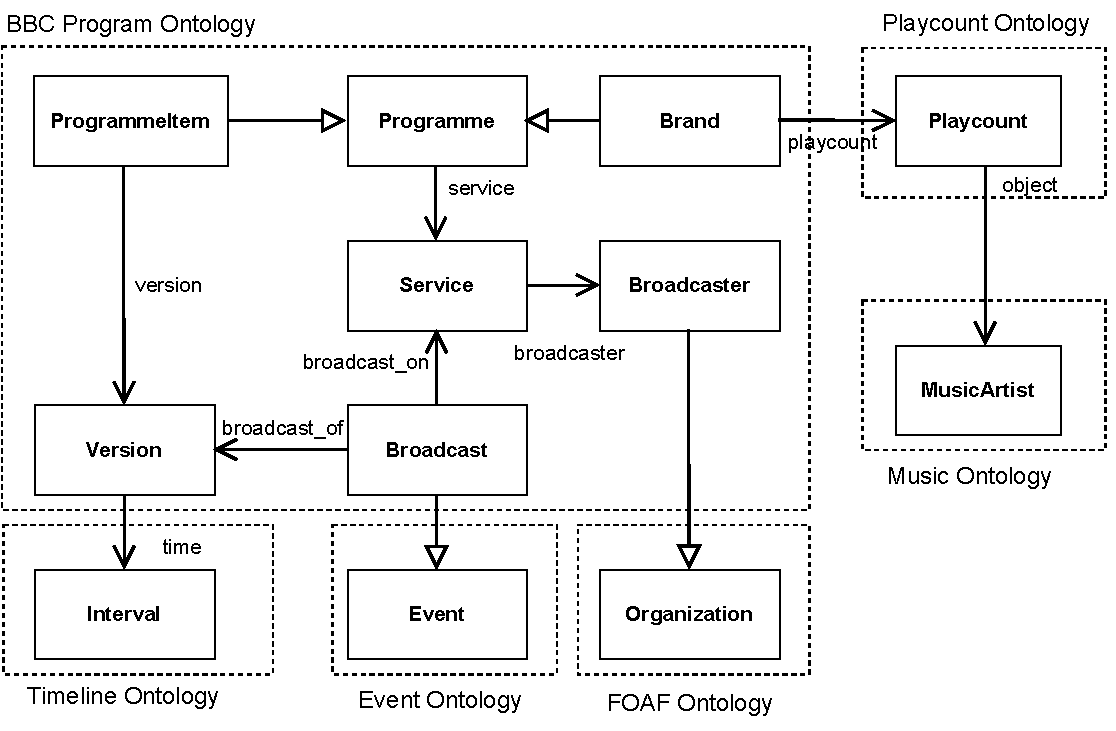
\includegraphics[scale=0.7]{figs/bbc-ontology-example-en}
   \caption{Example of the BBC ontology with links to other ontologies (notation based on UML, here without prefix for namespaces).}
   \label{fig:bbc-ontology-example}
\end{figure}

As all this data is available and interconnected by ontologies, a user of the Semantic Web can directly ask for answers to questions in this and other scenarios.
To make this possible, the Semantic Web requires generic software components, languages, and protocols that can interact seamlessly with each other.
We introduce the classical and modern components of the architecture of the Semantic Web in Section~\ref{sec:swarchitecture}.

In addition to the above example, the Semantic Web can be used for a variety of other applications (see examples in Section~\ref{sec:userinterfaces}).
Apart from technical aspects, the Semantic Web should also be understood as a socio-political phenomenon.
Similar to the World Wide Web, various individuals and organizations publish their data on the Semantic Web and collaborate to link and improve this data.
This impact on practitioners is discussed in Section~\ref{sec:impact}.

\section{Architecture of the Semantic Web}
\label{sec:swarchitecture}

The example in Section~\ref{sec:musicscenario} describes \emph{what} the Semantic Web is as an infrastructure, but not \emph{how} this is achieved.
In fact, the capabilities of the Semantic Web \emph{in a small scale} have already been implemented by some knowledge-based systems originating from artificial intelligence research, e.\,g., Heinsohn et al~\cite{DBLP:journals/ai/HeinsohnKNP94}.
However, for the implementation of the vision \emph{on a large scale}, i.\,e, the Web, these knowledge-based systems lacked flexibility, robustness, and scalability.
In part, this was due to the complexity of the algorithms used.
For example, knowledge bases in description logic in the 1990s, which serve as the basis of Web ontologies, were limited regarding their size such that they could handle at the most some hundred concepts~\cite{DBLP:journals/ai/HeinsohnKNP94}.

In the meantime, enormous improvements have been achieved.
Greatly increased computational power and optimized algorithms allow a practical handling of large ontologies like 
Simple Knowledge Organization System (SKOS)\myurl{https://www.w3.org/TR/skos-reference/}, 
Gene Ontology\myurl{https://geneontology.org/}, Schema.org, and SNOMED-CT\myurl{https://www.snomed.org/}.
However, there are some fundamental differences between traditional knowledge-based systems and the Semantic Web.
Data management in traditional knowledge-based systems has weaknesses in terms of handling large amounts of data and data sources, among other things because of 
different underlying formalisms,
distributed locations, 
different authorities,
different data quality, and 
a high frequency of change in the data used.

The Semantic Web applies fundamental principles to deal with these problems; they represent the basis for the architecture of the Semantic Web.
This architecture's building blocks can roughly be categorized into groups, covering the entire life cycle of handling and managing graph data on the Web.
These groups are
graph data representation,
creation and validation of graph data,
reasoning over and linking of graph data,
(distributed) querying of graph data, 
crypto, provenance, and trustworthiness of graph data, and
user interfaces and applications.

Below, we first introduce the principles of the Semantic Web, from which we derive the architecture and its main components.
Subsequently, we describe the groups of the architecture.
The principles of the Semantic Web are:

\begin{enumerate}
\item \emph{Explicit and simple data representation:}
A general data representation abstracts from the underlying formats and captures only the essentials.

\item \emph{Distributed systems:}
A distributed system operates on a large set of data sources without centralized control that regulates which information belongs where and to whom.

\item \emph{Cross-references:}
The advantages of a network of data in answering queries are not based solely on the sheer quantities of data but on their interconnection, which allows reusing data and data definitions from other sources.

\item \emph{Loose coupling with common language constructs:}
The World Wide Web and likewise the Semantic Web are mega-systems, i.\,e., systems consisting of many subsystems, which are themselves large and complex.
In such a mega-system, individual components must be loosely coupled in order to achieve the greatest possible flexibility.
Communication between the components is based on standardized protocols and languages, whereby these can be individually adapted to specific systems. 

\item \emph{Easy publishing and easy consumption:}
Especially in a mega-system, participation, i.\,e., publishing and consumption of data, must be as simple as possible.
\end{enumerate}
These principles are achieved through a mix of protocols, language definitions, and software components.
Some of these components have already been standardized by the W3C, which has defined both syntax and formal semantics of languages and protocols. 
Other components are not yet standardized, but they are already provided for the so-called \emph{Semantic Web Layer Cake} by Tim Berners-Lee (cf.~{\tt http://www.w3.org/2007/03/layerCake.png}).
We present a variant of the Semantic Web architecture, distinguishing between standardized languages and current developments.
A graphical representation of the architecture can be found in Figure~\ref{fig:layercake}.

\begin{figure}[ht]
  \centering
 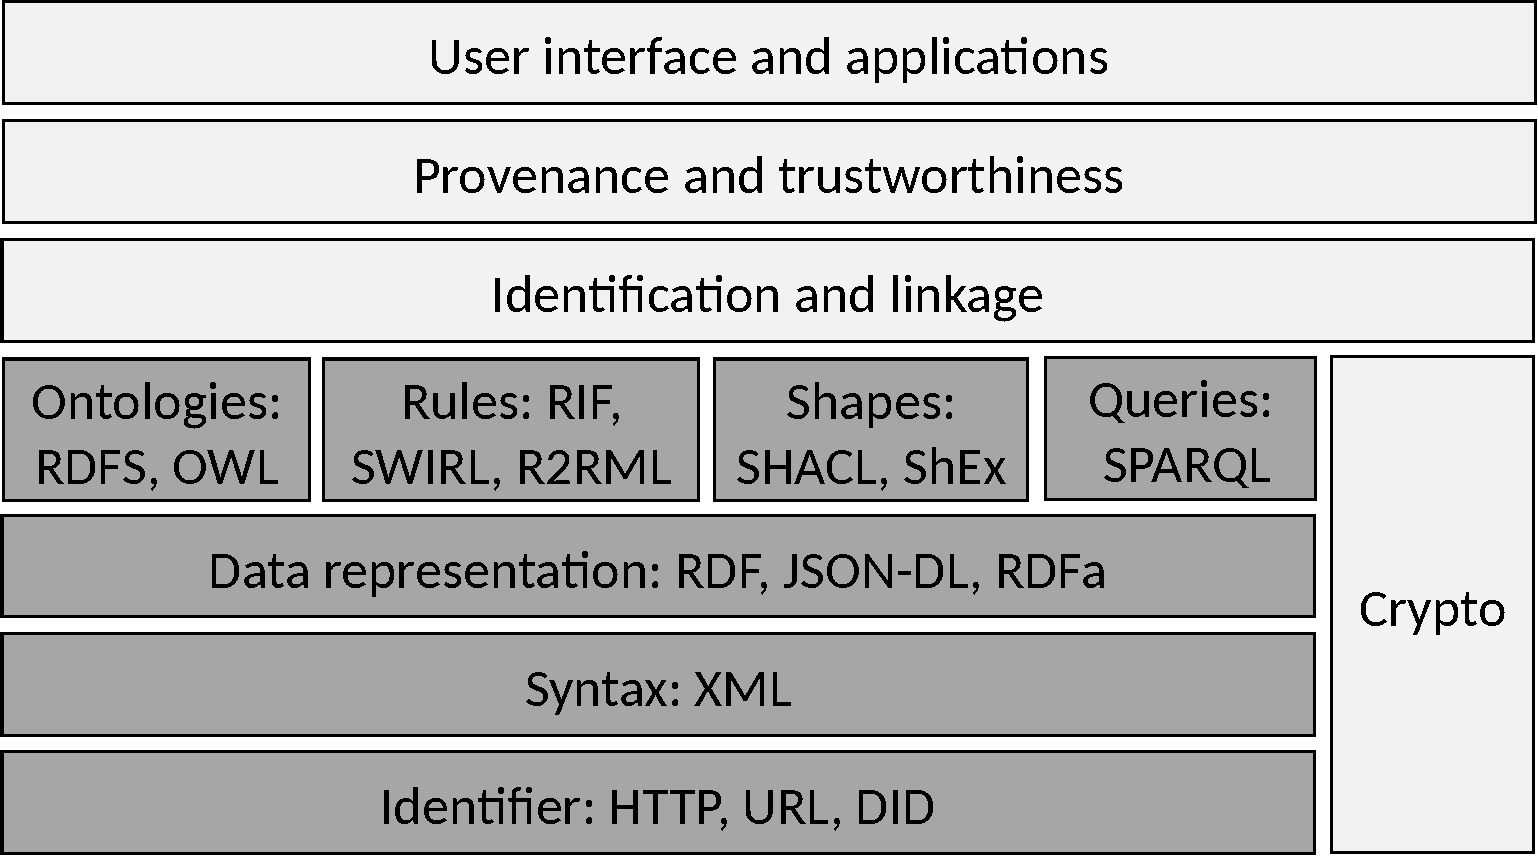
\includegraphics[width=0.75\textwidth]{figs/layer-cake-en-cropped.pdf}
 \caption{Representation of the components of the so-called ``Semantic Web Layer Cake''. W3C language standards are shown in dark gray. Current developments are shown in light gray.}
  \label{fig:layercake}
\end{figure}
 
\paragraph*{Identifier for Resources: HTTP, URL, DID}
Entities (also called resources) are identified on the Internet by so-called Uniform Resource Identifiers (URIs)~\cite{rfc1630}.
When a URI holds a dereferenceable location of the resource, in other words, it can be employed to get access to the resource via HTTP, it is called a Uniform Resource Locator (URL)~\cite{rfc1738,rfc3986}.
Furthermore, Internationalized Resource Identifiers (IRIs)~\cite{rfc3987} supplement URIs with international character sets from Unicode/ISO10646.
URIs are globally and universally used but are usually not under our control.
A recent W3C recommendation, the Decentralized Identifiers (DIDs), introduces an alternative approach to the above identifiers~\cite{w3c-did}.
A DID is by default decentralized and allows for self-sovereign management of the identity, i.\,e., the control of a DID and its associated data is with the users.

In our example in Section~\ref{sec:musicscenario}, a URI \footnote{\url{http://www.bbc.co.uk/music/artists/2f031686-3f01-4f33-a4fc-fb3944532efa#artist}} describes the musician Benny Andersson of the Swedish pop group ABBA.
A user can dereference a URI that refers to ABBA, e.\,g., by performing a so-called look-up using HTTP to obtain a detailed description of the URI.
We refer to the referenced standards for details.

For a detailed discussion of the role of dereferenceable URIs on the Semantic Web, we refer to the Linked Data principles described in Section~\ref{sec:linked-graph-data}.
 
\paragraph*{Syntax for Data Exchange: XML, JSON-LD, RDFa} 
The Extensible Markup Language (XML)\myurl{https://www.w3.org/TR/xml/} is used to structure documents and enables the specification and serialization of structured data. In addition, other data formats were introduced to facilitate for serialization of RDF data, often replacing XML.
We can view those formats as forming two groups.
The first group consists of formats designed specifically for RDF data, such as Turtle\myurl{https://www.w3.org/TR/turtle/}, N-triple\footnote{\url{https://www.w3.org/TR/n-triples/}}, and TRIG\myurl{https://www.w3.org/TR/trig/}.
These are easier to view in a text editor, compared to XML, and thus easier to understand and modify.
While initially not included in standards, their popularity has led to them being official W3C recommendations since 2014.
The other group of formats is built by extending existing data formats.
As a result, those can be employed to add RDF to existing systems.
Examples of such formats are JSON-LD\myurl{https://www.w3.org/TR/json-ld/}, CSV on the Web (CSVW)\myurl{https://www.w3.org/TR/tabular-data-primer/}, and RDFa\myurl{https://www.w3.org/TR/rdfa-primer/} extending JSON, CSV, and (X)HTML, respectively.

\paragraph*{Graph Data Representation: RDF}

In addition to the referencing of resources and a uniform syntax for the exchange of data, a data model is required that allows resources to be described both individually and in their entirety and how they are linked~\cite{DBLP:books/crc/linked2014,DBLP:reference/bdt/HartigHS19}.
An integrated representation of data from multiple sources is provided by a data model based on directed graphs~\cite{key:oem}.
The corresponding W3C standard language is RDF (Resource Description Framework)\footnote{\url{https://www.w3.org/RDF/}}.

An RDF graph consists of a set of RDF triples, where a triple consists of a subject, predicate (property), and object.
An RDF graph can be given an identifier, such a graph is called a named graph~\cite{DBLP:conf/semweb/CarrollBHS04}.
RDF graphs can be serialized in several ways (see Syntax for Data Exchange above).
It is important to note that some formats (e.\,g., Turtle) do not support named graphs. 
Finally, RDF-star (aka RDF*)\footnote{\url{https://w3c.github.io/rdf-star/}}$^,$\footnote{\url{https://blog.liu.se/olafhartig/2019/01/10/position-statement-rdf-star-and-sparql-star/}} was introduced to allow nesting of triples and thus enables an efficient way to make statements about statements while avoiding reification and the increased number of triples and complexity that come along with it.

The representation of graph data is further discussed in Section~\ref{sec:representation}.

\paragraph*{Creation and Validation of Graph Data: RIF, SWRL, [R2]RML, and SHACL}

In the RDF context, a rule is a logical statement employed to infer new facts from existing graph data or to validate the data itself.
RIF (Rule Interchange Format)\myurl{http://www.w3.org/2005/rules/wiki/RIF_Working_Group} is a W3C recommendation format designed to facilitate the seamless interchange of rules between different rule engines.
This enables the extraction of rules from one engine, their translation into RIF, publication, and subsequent conversion into the native syntax of another rule engine for execution.
SWRL\myurl{https://www.w3.org/submissions/SWRL/} is a rule-based language designed for representing complex relationships 
and reasoning.

Rules can also be used to state the correspondence between data sources and RDF graphs. 
The RDB to RDF Mapping Language (R2RML)\myurl{https://www.w3.org/TR/r2rml/} and the RDF Mapping Language (RML)\myurl{https://rml.io/specs/rml/} correspond to rule-based mapping languages for the declarative definition of RDF graphs. R2RML is the W3C recommendation for representing mappings from relational databases to RDF datasets, while RML extends R2RML to express rules not only from relational databases but also from data in the format of CSV, JSON, or XML.

Validating constraints, representing syntactic and semantic restrictions in RDF graphs, is essential for ensuring data quality.
In addition to rule-based languages, shapes allow for the specification of conditions to meet data quality criteria and integrity constraints.
A shape encompasses a conjunction of constraints representing conditions that nodes in an RDF graph must satisfy~\cite{DBLP:series/synthesis/2021Hogan}. 
A shapes graph is a labeled directed graph where nodes correspond to shapes, and edges denote interrelated constraints. 
The Shapes Constraint Language (SHACL)~\cite{SHACL} and Shape Expressions (ShEx)~\cite{SHEX}) are two W3C-recommendations  to express shapes graphs over RDF~\cite{DBLP:conf/www/RabbaniLH22}.

The creation and validation of graph data are described in detail in Section~\ref{sec:creation}.
\arxivonly{We introduce OWL and reasoning on graph data below.}

\paragraph*{Reasoning and Linking of Graph Data: RDFS, OWL}

Data from different sources may be heterogeneous. 
In order to deal with this heterogeneity and to model the semantic relationships between resources, the RDF Schema (RDFS)\myurl{https://www.w3.org/TR/rdf11-schema/} vocabulary extends RDF by modeling types of resources (so-called RDF classes) and semantic relationships on types and properties in the form of generalizations and specializations.
Likewise, it can be used to model the domain and range of properties.

RDFS is not expressive enough to merge data from different sources and define consistency criteria about it, such as the disjointness of classes or the equivalence of resources.
The Web Ontology Language (OWL)\myurl{https://www.w3.org/OWL/}~\cite{key:owl2} is an ontology language with formally defined meaning based on description logic.
This allows for reasoning services to be provided by knowledge-based systems for OWL ontologies. 
OWL can be exchanged using RDF data formats.
Compared to RDFS, OWL provides more expressive language constructs.
For example, OWL allows the specification of equivalences between classes and cardinality constraints on properties~\cite{key:owl2}.

Reasoning over RDF graphs, incorporating RDFS and OWL  models enhances semantic expressiveness and inferential capabilities. 
This involves making implicit information explicit, inferring new triples, and validating the RDF graph's consistency against defined ontological constraints. RDFS provides basic entailment regimens, creating hierarchies and simple inferencing via sub-class and sub-property relationships. In contrast, OWL introduces advanced constructs such as property characteristics (e.\,g., functional, inverse, symmetric properties), cardinalities, and disjointness axioms, enabling more expressive and complex modeling. Integrating RDFS and OWL reasoning mechanisms empowers applications to derive insights, discover implicit knowledge, and ensure adherence to specified ontological constraints within RDF-based knowledge representations. 

Graph data aggregated from many data sources, such as in our example in Section~\ref{sec:musicscenario}, may contain many different identities.
But those identities may represent the same set of real-world objects.
Integration and linkage mechanisms allow references to be made between data from different sources.
A popular approach to state the identity of two resources $v$ and $w$ is the \texttt{owl:sameAs} feature of OWL.

We discuss the reasoning over and linking of graph data in Section~\ref{sec:reasoning}.

\paragraph*{Querying of Graph Data: SPARQL}
Since RDF makes it possible to integrate data from different sources, a query language is needed that allows formulating queries over individual RDF graphs as well as over the combination of multiple RDF graphs across multiple sources. 
SPARQL\myurl{http://www.w3.org/TR/rdf-sparql-query/} (a recursive acronym for SPARQL Protocol and RDF Query Language) is a declarative query language for RDF graphs that enables us to formulate such queries. 
SPARQL~1.1\myurl{http://www.w3.org/TR/sparql11-query/} is the current version of SPARQL, which includes the capability to formulate federated queries over distributed data sources. 

The basic building blocks of a SPARQL query are triple and graph patterns. 
A triple pattern corresponds to an RDF triple but where one, two, or all three of its components are replaced by variables (denoted with a leading ``?''). 
These triple patterns with variables are to be matched in the queried graph.
Multiple triple patterns can be combined into more complex graph patterns describing the connections between multiple nodes in the graph. 
The solution to such a SPARQL query then corresponds to all the subgraphs in an RDF graph matching this pattern.

Finally, there is RDF-star (aka RDF*)\footnote{\url{https://w3c.github.io/rdf-star/}}$^,$\footnote{\url{https://blog.liu.se/olafhartig/2019/01/10/position-statement-rdf-star-and-sparql-star/}} -- along with the corresponding SPARQL-star/ SPARQL* extension -- was proposed and since then was implemented by several triple stores~\cite{AbuAebAgl23} that often provide publicly accessible SPARQL endpoints.
The key idea with RDF/SPARQL-star is to allow the nesting of triples to enable an efficient way to allow statements about statements while avoiding reification and the increased number of triples and complexity that come along with it.

We describe SPARQL and federated querying in Section~\ref{sec:distributeddataquerying}.

\paragraph*{Crypto, Provenance, and Trustworthiness of Graph Data}

Other aspects of the Semantic Web are encryption and authentication to ensure that data transmissions cannot be intercepted, read, or modified.
Crypto modules, such as SSL (Secure Socket Layer), verify digital certificates and enable data protection and authentication.
In addition, there are digital signatures for graphs that integrate seamlessly into the architecture of the Semantic Web and are themselves modeled as graphs again~\cite{DBLP:conf/esws/KastenSS14}.
This allows graph signatures to be applied iteratively and enables to building trust networks.
The Verifiable Credentials Data Model, a recent W3C recommendation, introduces a standard to model trustworthy credentials for graphs on the web\myurl{https://www.w3.org/TR/vc-data-model/}.
Data on the Semantic Web can be augmented with additional information about its trustworthiness and provenance.

Aspects of trustworthiness and provenance of graph data as well as crypto are discussed in Section~\ref{sec:trustprovenance}.

\paragraph*{User Interfaces and Applications}
A user interface enables users to interact with data on the Semantic Web.
From a functional perspective, some user interfaces are generic and operate on the graph structure of the data, whereas others are tailored to specific tasks, applications, or ontologies. 
New paradigms are exploring the spectrum of possible user interfaces between generality and specific end-user requirements.

Semantic Web applications are discussed in Section~\ref{sec:userinterfaces}.
The impact on practitioners is described in Section~\ref{sec:impact}.

\section{Representation of Graph Data}
\label{sec:representation} 

The Linked Open Data principles are notably the most successful and widely adopted choice for representing RDF graph data on the web.
Thus, we first introduce the reader to how to represent graph data as Linked Data.
Subsequently, we introduce the notion of ontologies. 
This is followed by a more detailed analysis of the different types of ontologies.
We give examples of ontologies throughout the sections.
With this background in mind, we reconsider our running example from Section~\ref{sec:musicscenario} and analyze the given distributed network of ontologies. 
In this context, we also introduce and discuss the notion of ontology design patterns.

\subsection{Linked Graph Data on the Web}
\label{sec:linked-graph-data}
The \emph{Linked Data} principles\myurl{http://www.w3.org/DesignIssues/LinkedData.html} define the methods for representing, publishing, and using data on the Semantic Web.
They can be summarized as follows:
\begin{enumerate}
\item URIs are used as names for entities.
\item The HTTP protocol's GET method is used to retrieve descriptions for a URI.
\item Data providers shall return relevant information in response to HTTP GET requests on URIs using standards, e.\,g., in RDF.
\item Links to other URIs shall be used to facilitate knowledge discovery and use of additional information.
\end{enumerate}
Publishing data using Linked Data principles allows easy access to data via HTTP.
This allows exploration of resources and navigation across resources on the Semantic Web.
URIs (see 1.) are dereferenced using HTTP requests~(2.) to obtain additional information about a given resource.
In particular, using standardized syntax~(3.), this information may also contain links to other resources~(4.).

Figure~\ref{fig:abba_linked_data} represents an example of Linked Data about the pop group ABBA.
The example describes several relationships linking entities to ABBA's URI, such as {\tt foaf:member} and {\tt rdf:type}.
In the figure ``ABBA'', or more precisely the URI of ABBA, is the subject, ``Property'' refers to relationships, and ``Value'' represents objects of the RDF triples.
The relation {\tt owl:sameAs} will be explained in more in Section \ref{sec:reasoning}. 
The prefixes \texttt{foaf}, \texttt{rdf}, and \texttt{owl} refer to vocabularies of the FOAF ontology\myurl{http://xmlns.com/foaf/spec/}, and the W3C language specifications of RDF and OWL, respectively.
\begin{figure}[ht]
  \centering
  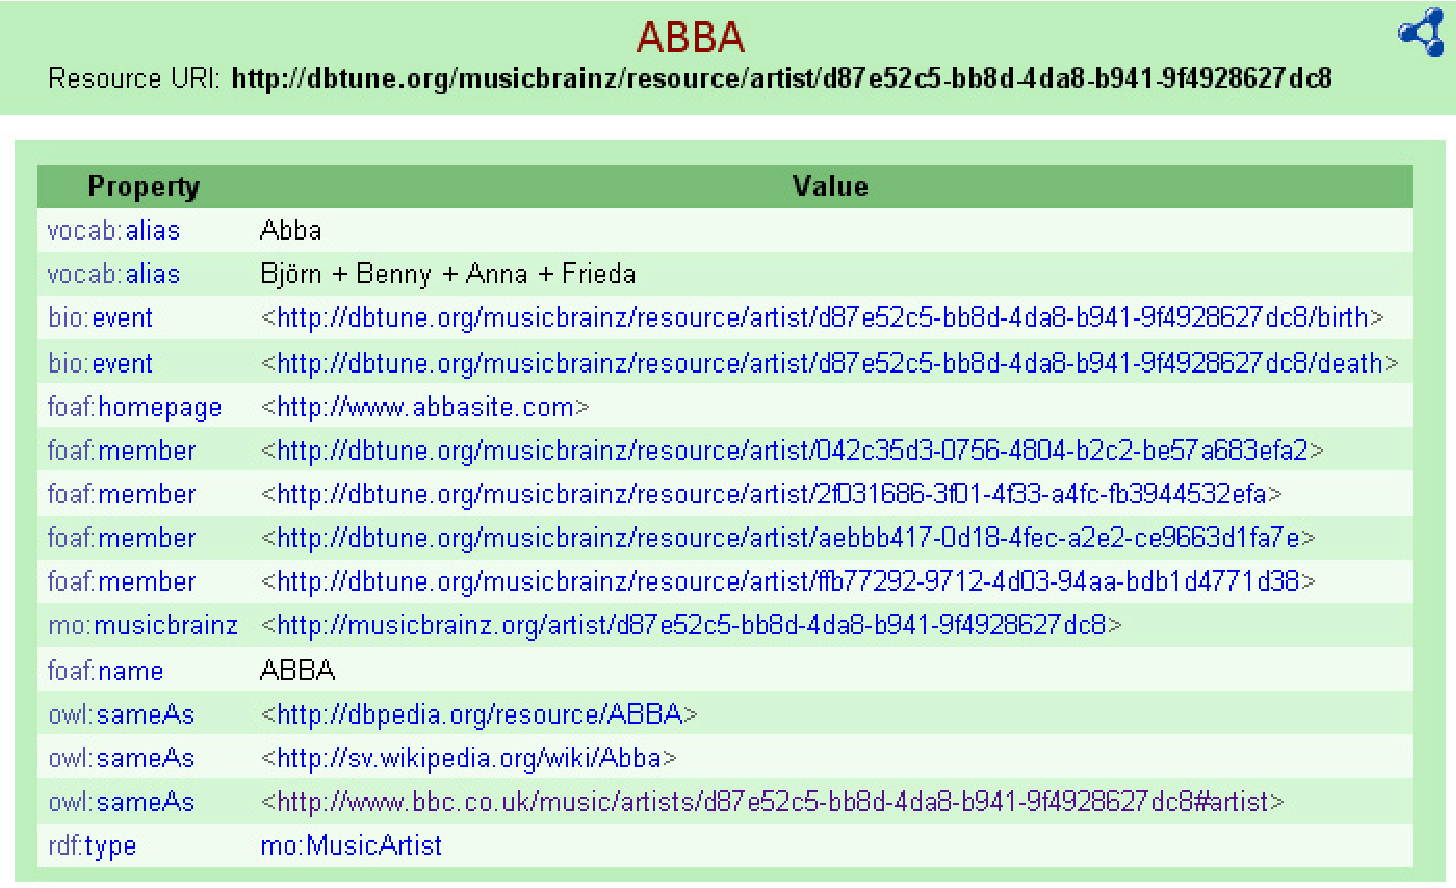
\includegraphics[width=\textwidth]{figs/abba-linked-data}
\caption{Linked Data example for ABBA.}\label{fig:abba_linked_data}
\end{figure}

\subsection{Ontologies}
\label{sec:ontologies:definition}

An ontology is commonly defined as a formal, machine-readable representation of key concepts and relationships within a specific domain~\cite{GuarinoOberleStaabWhatIsAnOntology2009,OberleMiddleware2006}.
In essence, ontologies capture a shared perspective~\cite{GuarinoOberleStaabWhatIsAnOntology2009} that is, the formal conceptualization of ontologies expresses a consensus view among different stakeholders. 
Visualizing ontologies is akin to viewing a spectrum, with a specificity of concepts, their relationships, and the granularity of meaning representation varying along this continuum
~\cite{DBLP:conf/dagstuhl/McGuinness03,DBLP:journals/sigmod/UscholdG04,DBLP:journals/ao/Uschold15}.
A controlled vocabulary corresponds to the less expressive form of ontology, comprising a restrictive list of words or terms used for labeling, indexing, or categorization. The Clinical Data Interchange Standards Consortium (CDISC) Terminology is an exemplary vocabulary that harmonizes definitions in clinical research.\myurl{https://datascience.cancer.gov/resources/cancer-vocabulary/cdisc-terminology} 
A thesaurus is located next in the spectrum; they enhance controlled vocabularies with information about terms and their synonyms and broader/narrower relationships. The Unified Medical Language System (UMLS) integrates medical terms and their synonyms.\myurl{https://www.nlm.nih.gov/research/umls/index.html}
Next, taxonomies are built over controlled vocabularies to provide a hierarchical structure, e.\,g., parent/child relationship. 
SNOMED-CT\myurl{https://www.snomed.org/value-of-snomedct} (Systematized Nomenclature of Medicine Clinical Terms) provides a terminology and coding system used in healthcare and medical fields; medical concepts organized in a hierarchical structure enabling a granular representation of clinical information. 
The Simple Knowledge Organization System (SKOS)\myurl{https://www.w3.org/TR/skos-reference/} is a W3C standard to describe knowledge about organizational systems. 
Lastly, ontologies are at the highest extreme of the spectrum, integrating sets of concepts with attributes and relationships to define a domain of knowledge.

Note, SKOS is a popular standard for modeling domain-specific taxonomies in the different scientific communities such as economics, social sciences, etc. to represent concepts and their relationships, most importantly narrower, broader, and related. However, it does not have the expressiveness of OWL with its complex expressions on classes and relations. For a detailed discussion, we refer to the literature such as~\cite{DBLP:conf/owled/JuppBS08} and the W3C on using OWL and SKOS\myurl{https://www.w3.org/2006/07/SWD/SKOS/skos-and-owl/master.html}.

\subsection{Types and Examples of Ontologies}
\label{sec:ontologies}

A network of ontologies, such as the example shown in Figure~\ref{fig:bbc-ontology-example}, may consist of a variety of ontologies created by different actors and communities. 
Ontologies may be the result of a transformation or reengineering activity of a legacy system, such as a relational database or existing taxonomy such as the Dewey Decimal Classification\myurl{http://dewey.info/} or Dublin Core.
Other ontologies are created from scratch.
This involves applying existing methods and tools for ontology engineering and choosing an appropriate representation language for the ontology (see Section~\ref{sec:reasoning}). 

Ontology engineering deals with the methods for creating ontologies~\cite{GomezPerezFernandezLopezOntologicalEngineering} and has its origins in software engineering in the creation of domain models and in database design in the creation of conceptual models.
A good overview of ontology engineering can be found in several reference books~\cite{GomezPerezFernandezLopezOntologicalEngineering}.
Ontologies vary greatly in their structure, size, development methods applied, and application domains considered. 
Complex ontologies are also distinguished in terms of their purpose and granularity.

\textbf{Domain Ontologies} represent knowledge specific to a particular domain~\cite{Euzenat2007a,OberleMiddleware2006}. 
Domain ontologies are used as external sources of background knowledge~\cite{Euzenat2007a}.
They can be built on foundational ontologies~\cite{Oberle:2007:DES:1290204.1290385} or core ontologies~\cite{ScherpEtAlDesigningCoreOntologiesIOS2011}, which provide precise structuring to the domain ontology and thus improve interoperability between different domain ontologies.
Domain ontologies can be simple such as the FOAF ontology or the event ontology mentioned above, or very complex and extensive, having been developed by domain experts, such as the SNOMED medical ontology.

\textbf{Core Ontologies} represent a precise definition of structured knowledge in a particular domain spanning multiple application domains~\cite{ScherpEtAlDesigningCoreOntologiesIOS2011,OberleMiddleware2006}. 
Examples of core ontologies include core ontologies for software components and web services~\cite{OberleMiddleware2006}, for events and event relationships~\cite{emf-mtap}, or for multimedia metadata~\cite{www-m3o}.
Core ontologies should thereby build on foundational ontologies to benefit from their formalization and strong axiomatization~\cite{ScherpEtAlDesigningCoreOntologiesIOS2011}.
For this purpose, new concepts and relations are added to core ontologies for the application domain under consideration and are specialized by foundational ontologies.
 
\textbf{Foundational Ontologies} have a very wide scope and can be reused in a wide variety of modeling scenarios~\cite{BorgoMasoloDOLCE2009}. 
They are therefore used for reference purposes~\cite{OberleMiddleware2006} and aim to model the most general and generic concepts and relations that can be used to describe almost any aspect of our world~\cite{BorgoMasoloDOLCE2009,OberleMiddleware2006}, such as objects and events.
An example is the Descriptive Ontology for Linguistic and Cognitive Engineering (DOLCE)~\cite{BorgoMasoloDOLCE2009}.
Such basic ontologies have a rich axiomatization that is important at the developmental stage of ontologies.
They help ontology engineers to have a formal and internally consistent conceptualization of the world, which can be modeled and checked for consistency.
For the use of foundational ontologies in a concrete application, i.\,e., during the runtime of an application, the rich axiomatization can often be removed and replaced by a more lightweight version of the foundational ontology.

In contrast, domain ontologies are built specifically to allow automatic reasoning at runtime.
Therefore, when designing and developing ontologies, completeness and complexity on the one hand must always be balanced with the efficiency of reasoning mechanisms on the other.
In order to represent structured knowledge, such as the scenario depicted in Figure~\ref{fig:bbc-ontology-example}, interconnected ontologies are needed, which are spanned in a network over the Internet. 
For this purpose, the ontologies used must match and be aligned with each other.

\subsection{Distributed Network of Ontologies and Ontology Patterns}

A network of ontologies must be flexible with respect to the functional requirements imposed on it. 
This is because systems are modified, extended, combined, or integrated over time.
In addition, the networked ontologies must lead to a common understanding of the modeled domain.
This common understanding can be achieved through a sufficient level of formalization and axiomatization, and through the use of ontology patterns.
An ontology pattern, similar to a design pattern in software engineering, represents a generic solution to a recurring modeling problem~\cite{ScherpEtAlDesigningCoreOntologiesIOS2011}. 
Ontology patterns allow to select parts from the original ontology.
Either all or only certain patterns of an ontology can be reused in the network.
Thus, to create a network of ontologies, e.\,g., existing ontologies and ontology patterns can be merged on the Web.
The ontology engineer can drive or explicitly provide for the modularization of ontologies using ontology patterns.
Core ontologies represent one approach to designing a network of ontologies (see in detail~\cite{ScherpEtAlDesigningCoreOntologiesIOS2011}).
They allow to capture and exchange structured knowledge in complex domains.
Well-defined core ontologies fulfill the properties mentioned in the previous section and allow easy integration and smooth interaction of ontologies (see also~\cite{ScherpEtAlDesigningCoreOntologiesIOS2011}).
The networked ontologies approach leads to a flat structure, as shown in Figure~\ref{fig:bbc-ontology-example}, where all ontologies are used on the same level.
Such structures can be managed up to a certain level of complexity.

\begin{figure}[ht]
  \centering
   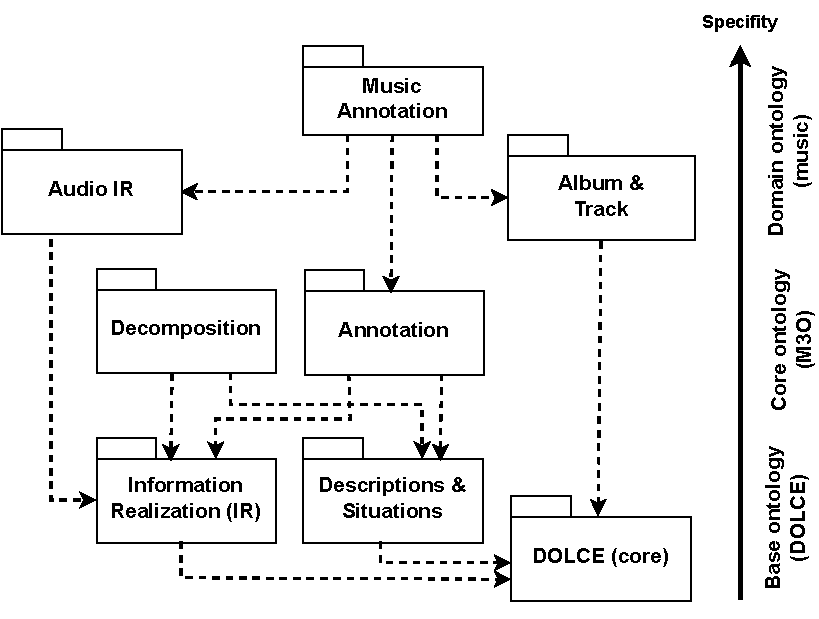
\includegraphics[scale=0.8]{figs/ontology-stack-en}
   \caption{Ontology layers combining the foundational ontology DOLCE, the multimedia metadata ontology M3O, domain-specific extensions to M3O for annotating audio data and music, and a domain ontology for albums and tracks.}
   \label{fig:ontology-stack}
\end{figure} 

The approach of networked core ontologies is illustrated by the example of ontology layers starting from foundational to core to domain ontologies.
As shown in Figure~\ref{fig:ontology-stack}, DOLCE is the foundational ontology at the bottom layer, the Multimedia Metadata Ontology (M3O)~\cite{www-m3o} as the core ontology for multimedia metadata, and an extension of M3O for the music domain.
Core ontologies are typically defined in description logic and cover a field larger than the specific application domain requires~\cite{GangemiPresuttiODP2009}. 
Concrete information systems will typically use only a subset of core ontologies.
To achieve modularization of core ontologies, they should be designed using ontology patterns.
By precisely matching the concepts in the core ontology with the concepts provided in the foundational ontology, they provide a solid foundation for future extensions.
New patterns can be added and existing patterns can be extended by specializing the concepts and roles.
Figure~\ref{fig:ontology-stack} shows different patterns of the M3O and DOLCE ontologies.

Ideally, the ontology patterns of the core ontologies are reused in the domain ontologies~\cite{GangemiPresuttiODP2009}, as shown in Figure~\ref{fig:ontology-stack}.
However, since it cannot be assumed that all domain ontologies are aligned with a foundational or core ontology, the option that domain ontologies are developed and maintained independently must also be considered.
In this case, domain knowledge can be reused in core ontologies by applying the Descriptions and Situations (DnS) ontology pattern of the foundational ontology DOLCE.
The DnS ontology pattern is an ontological formalization of context~\cite{OberleMiddleware2006} by defining different views using roles.
These roles can refer to domain ontologies and allow a clear separation of the structured knowledge of the core ontology and domain-specific knowledge.
To model a network of ontologies, such as the example described above, the Web Ontology Language (OWL) and its ability to axiomatize using description logic~\cite{DBLP:conf/dlog/2003handbook} is used.
In addition to being used to model a distributed knowledge representation and integration, OWL, is also used in particular to derive inferences from this knowledge, which is described in Section~\ref{sec:reasoning}.

\section{Creation and Validation of Graph Data}
\label{sec:creation}
In this section, we describe the creation of graph data from legacy data. 
Many tools are available for this task, which support various mappings and transformations.
Subsequently, we discuss data quality and the validation of knowledge graphs, including the recent approaches on shapes.
We also reflect on the role of the open-world versus closed-world assumption with respect to validating data.

\subsection{Graph Data Creation}
Graph data can be created by transforming legacy data via a data integration system~\cite{lenzerini2002data}, which consists of a unified schema, data sources, and mapping rules. 
These mapping rules define the concepts within the schema and establish links to the data sources.
By employing declarative definitions, knowledge graph creation promotes modularity and reusability.
This approach allows users to trace the entire graph creation process, leading to improved transparency and ease of maintenance.

To enable comprehensive and extensive graph specification, mappings and transformations have been developed to convert data from various storage models into Semantic Web data models like RDF. 
These mappings and transformations facilitate the mapping of data into RDF, thereby supporting the integration of diverse data sources into the Semantic Web.

The mapping language R2RML~\cite{W3CR2RML} defines mapping rules from relational databases (relational data models) to RDF graphs.
These mappings themselves are also RDF triples~\cite{W3TURTLE}. 
Because of its compact representation, Turtle is considered a user-friendly notation of RDF graphs.
The structure of R2RML is illustrated in Figure \ref{fig:r2rml}; essentially, table contents are mapped to triples by the classes \texttt{SubjectMap}, \texttt{PredicateMap}, and \texttt{ObjectMap}.
If the object is a reference to another table, this reference is called \texttt{RefObjectMap}. 
Here, \texttt{SubjectMap} contains primary key attributes of the corresponding table. 
Thus, there exists a mapping rule representable in RDF graphs by means of which tables of relational databases can be represented as RDF graphs.

\begin{figure}[ht]
  \centering
  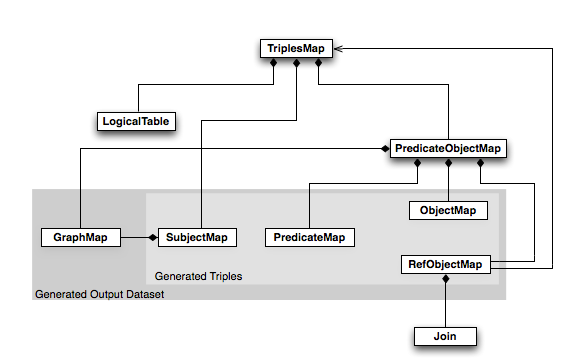
\includegraphics[width=1\textwidth]{figs/R2RML.PNG}
\caption{Structure of a relational data mapping (source: \cite{W3CR2RML}).}\label{fig:r2rml}
\end{figure}
 
The RDF Mapping Language (RML)\cite{DimouSCVMW14} extends R2RML to encompass the definition of logical sources in various formats, including CSV, JSON, XML, and HTML.
This enhancement enables RML to introduce new operators that facilitate the integration of data from diverse sources into the Semantic Web.
Thus, instead of \texttt{LogicalTable}, RML includes the tag \texttt{LogicalSource}, to allow for the retrieval of data in several formats.
Additionally, RML resorts to W3C-standardized vocabularies and enables the definition of retrieval procedures to collect data from Web APIs or databases. R2RML and RDF mapping rules are expressed in RDF, and their graphs document how classes and properties in one or various ontologies that are part of an RDF graph are populated from data collected from potentially heterogeneous data sources. 
 
Over time, the Semantic Web community has actively contributed to addressing the challenge of integrating heterogeneous datasets, resulting in the development of several frameworks for executing declarative mapping rules~\cite{chebotko2009semantics,calvanese2017ontop,DBLP:conf/www/PriyatnaCS14}.
A rich spectrum of tools (e.\,g., RMLMapper~\cite{DimouSCVMW14}, RocketRML~\cite{csimcsek2019rocketrml}, CARML\footnote{\url{https://github.com/carml/carml}}, SDM-RDFizer~\cite{iglesias2020sdm}, Morph-KGC~\cite{arenas2022morph}, and RMLStreamer~\cite{oo2022rmlstreamer}) offers the possibility of executing R2RML and RML rules and efficiently materializing the transformed data into RDF graphs.
Van Assche et\,al.~\cite{DBLP:journals/ws/AsscheDHHMD23} provided an extensive survey detailing the main characteristics of these engines.
Despite significant efforts in developing these solutions, certain parameters can impact the performance of the graph creation process~\cite{Chaves-FragaEIC19}.
Existing engines may face challenges when handling complex mapping rules or large data sources.
Nonetheless, the community continues to collaborate and address these issues.
An example of such collaboration is the Knowledge Graph Construction Workshop 2023 Challenge\footnote{\url{https://zenodo.org/record/7689310}} that took place at ESWC 2023.
This community event aims to understand the strengths and weaknesses of existing approaches and devise effective methods to overcome existing limitations.
 
RDF graphs can also be dynamically created through the execution of queries over data sources. These queries involve the rewriting of queries expressed in terms of an ontology, based on mapping rules that establish correspondences between data sources and the ontology. Tools such as Ontop~\cite{calvanese2017ontop}, Ultrawrap~\cite{DBLP:journals/ws/SequedaM13}, Morph~\cite{DBLP:conf/www/PriyatnaCS14}, Squerall~\cite{mami2019squerall}, and Morph-CSV~\cite{chaves2020enhancing} exemplify systems that facilitate the virtual creation of RDF graphs.

\subsection{Quality and Validation of Graph Data}
\label{sec:quality-and-validation}

Quality and validation of the graph data are crucial to maintaining the integrity of the Semantic Web~\cite{DBLP:journals/corr/abs-2308-14217,DBLP:journals/semweb/Debattista0AC18,Zaveri2015surveyQuality}. The evaluation of integrity constraints allows for the identification of inconsistencies, inaccuracies, or contradictions within the data. They also help maintain consistency by ensuring related data elements remain coherent. Constraints are logical statements -- expressed in a particular language -- that impose restrictions on the values taken for target nodes in a given property.

Constraints can be expressed using OWL~\cite{DBLP:conf/aaai/TaoSBM10}, SPARQL queries~\cite{DBLP:conf/edbt/LausenMS08}, or using shapes. However, the interpretation of the results depends on the semantics followed to interpret the failure of an integrity constraint. For example, constraints expressed in OWL are validated using an Open-World Assumption (OWA) (i.\,e., a statement cannot be inferred to be false based on failures to prove it) and under the absence of the Unique Name Assumption (UNA) (i.\,e., two different names may refer to the same object). These two features make it difficult to validate data in applications where data is supposed to be complete. Definitions of integrity constraint semantics in OWL using the Closed-World Assumption~\cite{Motik2007,Motik2009,DBLP:conf/aaai/TaoSBM10} overcome these issues.

Contrarily, constraints expressed using SPARQL queries or shapes will be evaluated under the Closed-World Assumption (CWA) and following the Unique Name Assumption (UNA). Nevertheless, some constraints may be difficult to express in SPARQL, and the specification process is prone to errors and difficult to maintain.
 
Data quality conditions and integrity constraints can also be expressed as graphs of shapes or the so-called \emph{shapes schema}. 
A shape corresponds to a conjunction of constraints that a set of nodes in an RDF graph must satisfy~\cite{DBLP:series/synthesis/2021Hogan}.
These constraints can restrict the types of nodes, the cardinality of certain properties, and the expected data types or values for specific properties. A shape can target the instances of a class, the domain or range of a property, or a specific node in the RDF graph. A shape or node in a shapes graph is validated in an RDF graph, if and only if, all the target nodes in the RDF graph satisfy all the constraints in the shape.
Figure~\ref{fig:shape} presents a shapes graph of three shapes targeting the classes  
\texttt{Brand}, \texttt{Playcount}, and \texttt{MusicArtist}. Each of the shapes comprises one constraint. In the shapes \texttt{Brand} and \texttt{MusicArtist} the properties title and name can take more than one value, while the shape \texttt{Playcount} states that each instance of the class \texttt{Playcount} must have exactly one value of the property \texttt{count}. Additionally, the instances of the class \texttt{Brand} must be related to valid instances of the class \texttt{Playcount} which should also be related to valid instances of the class \texttt{MusicArtist}.

\begin{figure}[!ht]
\centering
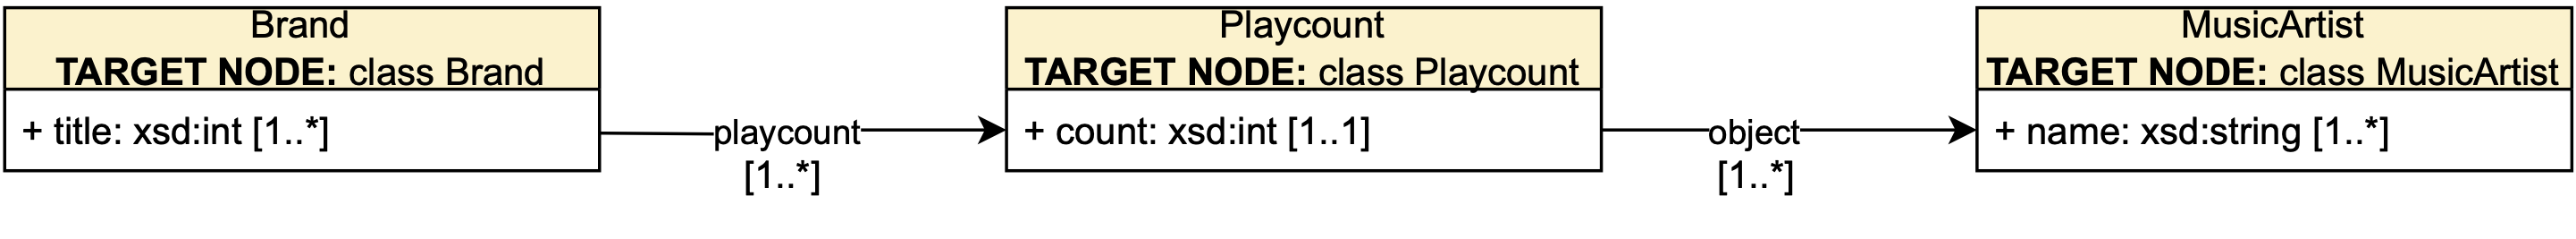
\includegraphics[width=1\textwidth]{figs/SHACLExample.png}
\caption{\textbf{Shapes for Graph Data.} A shapes graph comprises three shapes interlinked by the properties \texttt{playcount} and \texttt{objects} between the target classes \texttt{Brand}, \texttt{Playcount}, and \texttt{MusicArtist}.}
\label{fig:shape}
\end{figure}
  
There are two standards for defining shapes, ShEx (Shape Expressions)~\cite{SHEX}) and SHACL (Shapes Constraint Language)~\cite{SHACL}).
Both define shapes over the attributes (i.\,e., \texttt{owl:Datatype\-Properties}), and constraints on incoming/outgoing arcs, cardinalities, RDF syntax, and extension mechanism. These inter-class constraints induce a shape network used to validate the integrity and data quality properties of an RDF graph. 
 
SHACL and ShEx, although sharing a common goal, adopt distinct approaches. ShEx seeks to offer a language serving as a grammar or schema for RDF graphs, delineating RDF graph structures for validation. On the other hand, SHACL is positioned as the W3C recommendation for validating RDF graphs against a conjunction of constraints, emphasizing a constraint language for RDF. Despite their analogous roles in specifying shapes and constraints for RDF data, ShEx and SHACL differ in syntax, expressiveness, and community adoption \cite{DBLP:series/synthesis/2017Gayo}.

The evaluation results of a SHACL shape network over an RDF graph are presented in validation reports using a controlled vocabulary. A validation report includes explanations about the violations, the severity of the violation, and a message describing the violation. SHACL is the language selected by the International Data Space (IDS) to express the restrictions that state the integrity over RDF graphs \cite{DBLP:books/sp/22/0002LB22}. Besides the integrity validation of an RDF graph, SHACL can be utilized 
to describe data sources and the certification of a query answer \cite{DBLP:conf/vldb/Rohde21},
as metadata to enhance the performance of a SPARQL query engine \cite{DBLP:conf/edbt/RabbaniLH21},
to certify access policies \cite{DBLP:conf/esws/RohdeV23}, and 
to provide provenance as a result of the validation of integrity constraints~\cite{DBLP:conf/edbt/DelvaDJB23}. 

In the context of a quality assessment pipeline, one crucial step involves validating the shape schema against a graph. It is important to mention that the validation of recursive shape schemas is not explicitly addressed in the SHACL specification~\cite{SHACL}. 
To address this gap, Corman et al.~\cite{Corman2018} introduce a semantic framework for validating recursive SHACL. They also demonstrated that validating full SHACL features is an NP-hard problem. Building on these insights, they proposed specific fragments of SHACL that are computationally tractable, along with a fundamental algorithm for validating shape schemas using SPARQL~\cite{Corman2019}.
In a related vein, Andresel et al.~\cite{Andresel2020} propose a stricter semantics for recursive SHACL, drawing inspiration from stable models employed in Answer Set Programming (ASP). This innovative approach enables the representation of SHACL constraints as logic programs and leverages existing ASP solvers for shape schema validation. Importantly, this approach allows for the inclusion of negations in recursive validations. Further, Figuera et al.~\cite{DBLP:conf/www/FigueraRV21} present Trav-SHACL, an approach that focuses on query optimization techniques aimed at enhancing the incremental behavior and scalability of shape schema validation.

While SHACL has been adopted in a broad range of use cases, given a large graph it remains a challenge how to define shapes efficiently~\cite{DBLP:conf/www/RabbaniLH22}.
In many industrial settings with billions of entities and facts~\cite{Noy19} creating shapes manually simply is not an option. 
The current state of the art can automatically extract shapes on WikiData (ca. 2 Billion facts) in less than 1.5 hours while filtering shapes based on the well-established notions of support and confidence to avoid reporting thousands of shapes that are so rare or apply to such a small subset of the data that they become meaningless~\cite{DBLP:journals/pvldb/RabbaniLH23}.
Still, more work is needed to increase scalability further and also to help users make good use of the mined shapes~\cite{DBLP:conf/sigmod/RabbaniLH23} and, e.\,g., interactively use them to correct and improve the quality of their graphs.

\section{Reasoning over and Linking of Graph Data}
\label{sec:reasoning}

Section~\ref{sec:swarchitecture} introduced several formal languages for knowledge representation on the Semantic Web.
RDF allows the description of simple facts (statements with subject, predicate, and object, so-called RDF triples), e.\,g., ``Anni-Frid Lyngstad'' ``is a member of'' ``ABBA''.
RDFS allows the definition of types of entities (classes), relationships between classes, and a subclass and superclass hierarchy between types (analogously for relations).
OWL is even more expressive than RDF and RDFS.
For example, OWL allows the definition of disjoint classes or the description of classes in terms of intersection, union, and complement of other classes.

Below, we first introduce the reasoning over RDFS and OWL at the example of our BBC scenario from Section~\ref{sec:musicscenario}.
Subsequently, we discuss works on linking data objects and concepts.

\subsection{Reasoning over Graph Data}

Based on formal languages representing graph data and their semantics, further (implicit) facts can be derived from the knowledge base by deductive inference.
In the following, we exemplify the derivation of implicit facts from a set of explicitly given facts using the RDFS construct \texttt{rdfs:subClassOf} and the OWL construct \texttt{owl:sameAs}.
The property \texttt{rdfs:subClassOf} describes hierarchical relationships between classes and with \texttt{owl:sameAs} two resources can be defined as identical.

As a first example, we consider the class \texttt{foaf:Person}, which is defined in the FOAF ontology, and the classes \texttt{mo:Musician} and \texttt{mo:Group}, which are defined in the music ontology.
In the music ontology, there is an additional axiom that defines \texttt{mo:Musician} as a subclass of \texttt{foaf:Person} using \texttt{rdfs:subClassOf}.
Given this axiom, it can be deduced by deductive inference that instances of \texttt{mo:Musician} are also instances of \texttt{foaf:Person}.
Now if there is such a hierarchy of classes and in addition a statement that Anni-Frid Lyngstad is of type \texttt{mo:Musician}, then it can be inferred by inference that Anni-Frid Lyngstad is also of type \texttt{foaf:Person}.
This means that all queries asking for entities of type \texttt{foaf:Person} will also include Anni-Frid Lyngstad in the query result, even if that entity is not explicitly defined as an instance of \texttt{foaf:Person}.
Figure~\ref{fig:rdf-example-graph} represents these facts and the corresponding class hierarchy in RDFS as a directed graph.

\begin{figure}[ht]
  \centering
  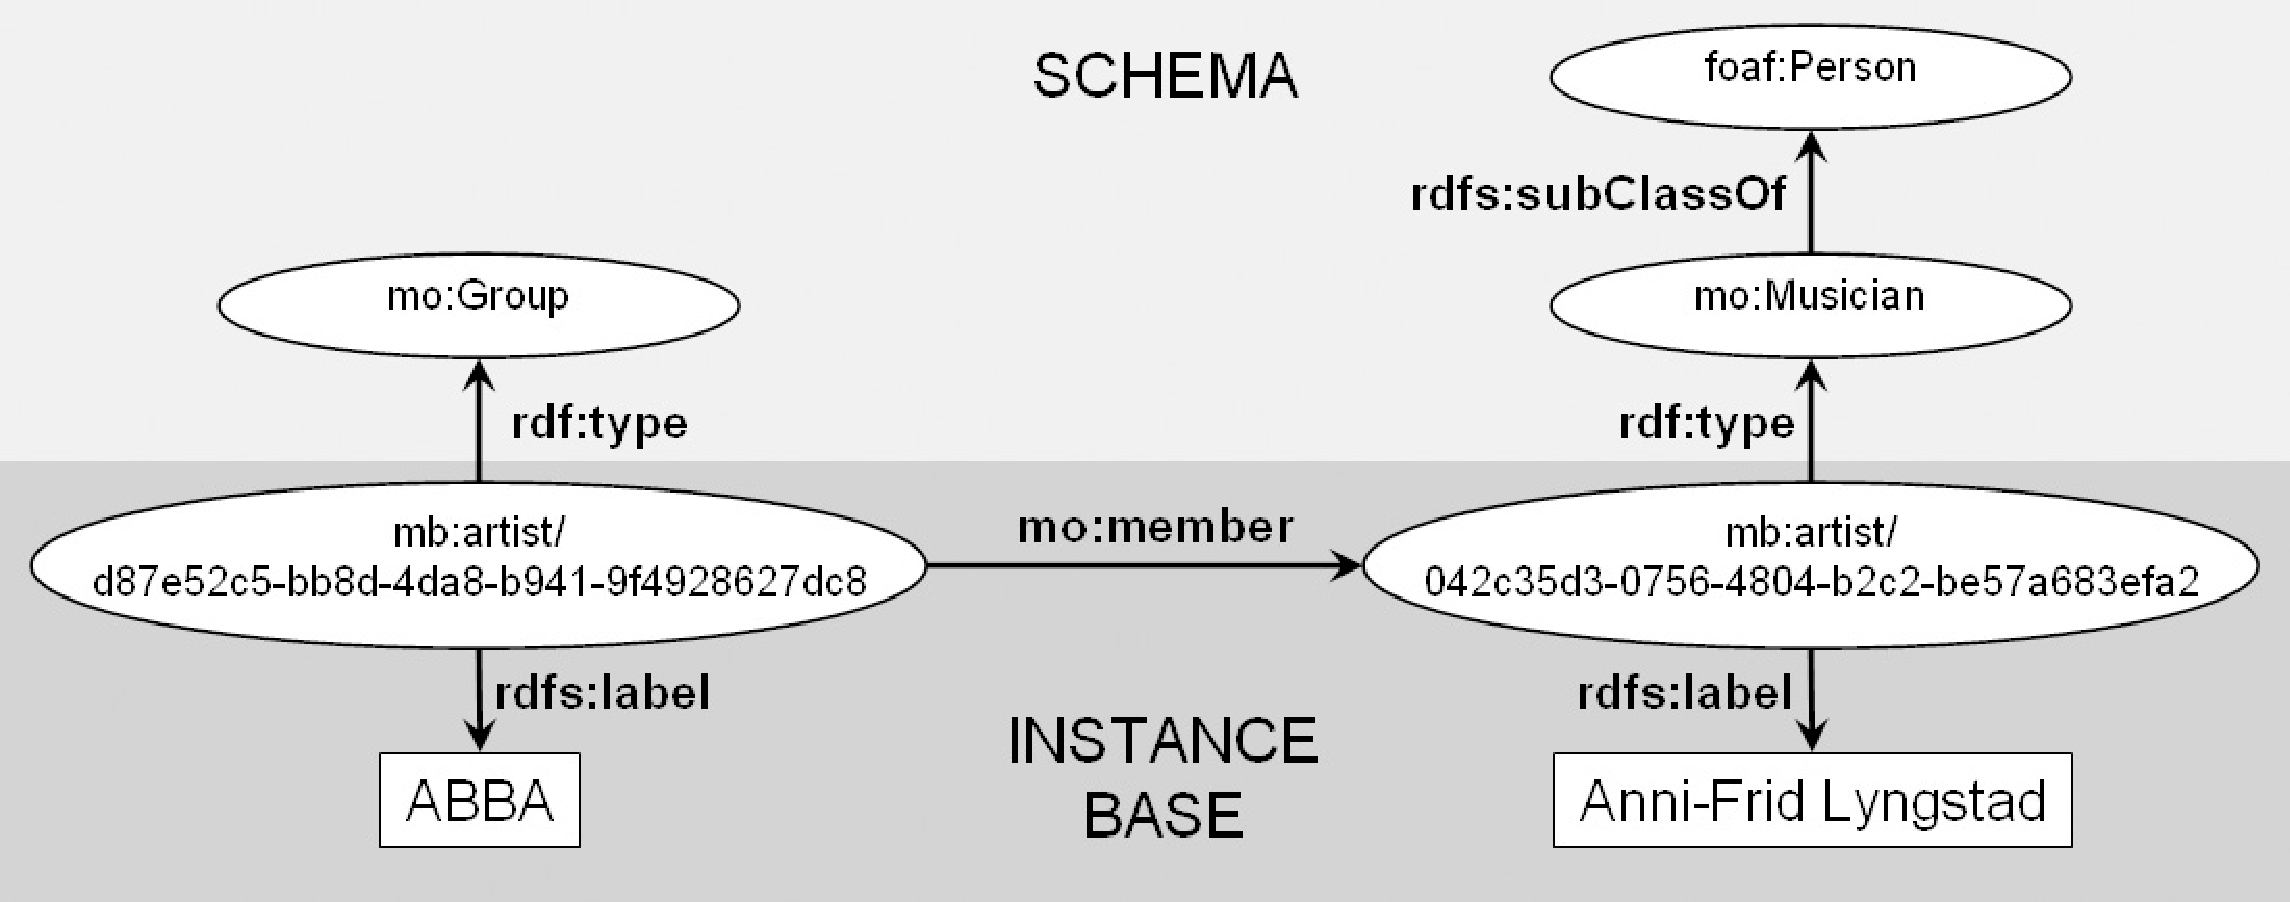
\includegraphics[width=0.9\textwidth]{figs/rdf-example-graph}
\caption{Visualization of RDF sample data about ABBA and Anni-Frid Lyngstad to illustrate inference in RDFS.}\label{fig:rdf-example-graph}
\end{figure}

In the second example, the OWL construct \texttt{owl:sameAs} is used to define two resources as identical, for example
\url{http://www.bbc.co.uk/music/artists/d87e52c5-bb8d-4da8-b941-9f4928627dc8#artist} and \url{http://dbpedia.org/resource/ABBA}.
Identical here means that these two URIs represent the same real-world object.
By inference, information about ABBA from different sources can now be linked.
Since ontologies are created independently on the web, and URIs are subject to local naming conventions, a real-world object may be represented by multiple URIs (in different ontologies).  

OWL offers a variety of other constructs for the description of classes, relationships, and concrete facts. 
For example, OWL allows the declaration of transitive relations and inverse relations. 
For example, the relation ``is-member'' is inverse to ``has-member''.
OWL reasoning allows, among other things, consistency checking of an ontology or checking the satisfiability of classes~\cite{DBLP:reference/sp/HorrocksP11}.
A class is satisfiable if there can be instances of that class.

For a detailed discussion about OWL reasoning, we refer to the literature such as~\cite{DBLP:reference/sp/HorrocksP11,DBLP:journals/sLogica/BaaderS01}.
Different reasoners for OWL have seen widespread adoption in the community such as the well-known Pellet\footnote{\url{https://github.com/stardog-union/pellet}} and Hermit~\cite{DBLP:journals/jar/GlimmHMSW14}.
Finally, a combination of description logic and rules is also possible.
For example, Motik et al.~\cite{DBLP:conf/semweb/MotikSS04} presented a combination of description logic and rules that allows tractable inference on OWL ontologies. 

\subsection{Linking of Objects and Concepts}
\label{sec:identity}

In the Semantic Web, it cannot be assumed that two URIs refer to two different real-world objects (cf. unique name assumption in Section~\ref{sec:quality-and-validation}).
A URI by itself, or in itself, has no identity~\cite{HalpinP09}.
Rather, the identity or interpretation of a URI is revealed by the context in which it is used on the Semantic Web.
Determining whether or not two URIs refer to the same entity is not a simple task and has been studied extensively in data mining and language understanding in the past.
For example, to identify whether or not the author names of research papers refer to the same person, it is often not sufficient to resolve the name, venue, title, and co-authors~\cite{PallikaEtAlCoreference2007}.
The process of determining the identity of a resource is often referred to as entity resolution~\cite{PallikaEtAlCoreference2007}, coreference resolution~\cite{WickEtAlCoreference}, object identification~\cite{RendleS06}, and normalization~\cite{WickEtAlCoreference,WickKDD2008}.
Correctly determining the identity of entities on the Web is important as more and more records appear on the Web and this presents a significant hurdle for very large Semantic Web applications~\cite{GlaserLOD2009}.

To address this, a number of services exist that can recognize entities and determine their identity:
Thomson Reuters offers OpenCalais\myurl{https://www.refinitiv.com/en/products/intelligent-tagging-text-analytics}, a service that can link natural language text to other resources using entity recognition. 
Another commercial tool that allows for extracting knowledge graphs from text is provided by DiffBot.\myurl{https://www.diffbot.com/}
Recently, the language model ChatGPT has been compared to the specialized entity and relation extraction tool REBEL~\cite{DBLP:conf/emnlp/CabotN21} for the task of creating knowledge graphs from sustainability-related text~\cite{DBLP:journals/corr/abs-2305-04676}.
The experiments suggest that large language models improve the accuracy of creating knowledge graphs~\cite{DBLP:journals/corr/abs-2305-04676}.
The sameAs\myurl{http://sameas.org/} service aims to detect duplicate resources on the Semantic Web using the OWL relationship \concept{owl:sameAs}.
This can be used to resolve coreferences between different datasets.
For example, for the query with the URI \url{http://dbpedia.org/resource/ABBA}, a list of over 100 URIs is returned that also references the music group ABBA.
One of them is BBC with the resource \url{http://www.bbc.co.uk/music/artists/d87e52c5-bb8d-4da8-b941-9f4928627dc8#artist}.

Furthermore, the problem of schema matching~\cite{WickKDD2008} is very related to the problem of entity resolution, co-reference resolution, and normalization.
The goal of schema matching is to address the question of how to integrate data~\cite{WickKDD2008}, which is non-trivial even for small schemas. 
In the Semantic Web, schema matching means the matching of different ontologies, respectively the concepts defined in these ontologies.
Various (semi-)automatic or machine learning techniques for matching ontologies have been developed in the past~\cite{euzenat2007b,Ehrig07,Blomqvist09}.
Core ontologies as illustrated in Figure~\ref{sec:ontologies} represent generic modeling frameworks for integration and alignment with other ontologies. 
In addition, core ontologies can also integrate Linked Open Data, which typically contains no or very little schema information.
The YAGO ontology~\cite{YagoWWW07} was generated from the fusion of Wikipedia and Wordnet using rule-based and heuristic methods.
A manual assessment showed an accuracy of 95\%.

Manual matching of different data sources is also pursued in the Linked Open Data project of the German National Library\myurl{http://www.d-nb.de/}.
For example, the database containing the authors of all documents published in Germany was manually linked with DBpedia and other data sources.
A particular challenge was to identify the authors, as described above.
For example, former German Chancellor Helmut Kohl has a namesake whose work should not be linked to the chancellor's DBpedia entry.
Relationships between keywords used to describe publications are asserted using the SKOS (Simple Knowledge Organization System) vocabulary.\myurl{https://www.w3.org/TR/2009/REC-skos-reference-20090818/}
For example, keywords are related to each other using the relation \concept{skos:related}.
Hyponyms and hypernyms are expressed by the relations \concept{skos:narrower} and \concept{skos:broader}.
Finally, the Ontology Alignment Evaluation Initiative\myurl{http://oaei.ontologymatching.org/} should be mentioned, which aims to achieve an established consensus for evaluating ontology matching methods.

\section{Querying of Linked Data}
\label{sec:distributeddataquerying}

Queries over Linked Data can be processed using link traversal~\cite{DBLP:conf/esws/Hartig11}, i.\,e., the query processor would use one of those IRIs given directly in the query as starting point and query the respective source for more triples involving the IRI. 
By iteratively doing this for more IRIs and with respect to the graph pattern defined in the query, a local set of triples is collected over which the given query can be evaluated.

More conveniently, queries over RDF and Linked Data can be formulated in SPARQL\footnote{\url{http://www.w3.org/TR/sparql11-query/}}, if a corresponding endpoint to the graph data is made available. 
Whereas such queries can target graphs that are stored in a single graph store, Linked Data often requires formulating and executing queries across multiple graphs that are stored at distributed data sources.

Below, we first introduce the basic query processing of SPARQL queries along with our running example.
This is followed by discussing RDFS/OWL entailment regimes and querying.
Finally, we present approaches for distributed querying over multiple SPARQL endpoints.

\subsection{Basic Query Processing}
\label{subsec:querying}

In principle, a SPARQL query is evaluated by comparing the graph pattern defined in the query to the RDF graph and reporting all matches as results. The set of results can be restricted by additional criteria, such as filters, i.\,e., conditions on variables and triple patterns that additionally need to be fulfilled.

As an example, let us consider the query illustrated in Figures~\ref{fig:spaqrl_abba_members_graph} and~\ref{fig:spaqrl_abba_members} that we want to execute over our example MusicBrainz graph from Section~\ref{sec:musicscenario}. 
We are now interested in the musicians of ABBA who are also members of other bands.
If we follow the Linked Data principles and evaluate the query using link traversal~\cite{DBLP:conf/esws/Hartig11}, this would mean first querying for triples including the IRI that represents ABBA, then navigating to the individual band members, and then following the links to all of the members' bands and query more relevant triples.

\begin{figure}[ht]
  \centering
  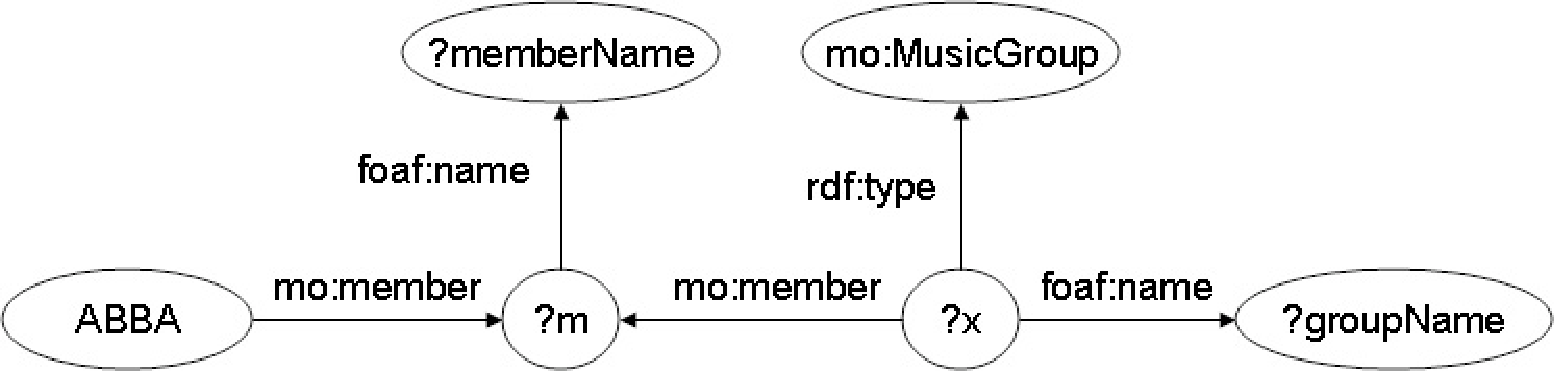
\includegraphics[width=0.8\textwidth]{figs/sparql-query}
\caption{Graphical representation of a query for music groups (represented by the variable \textit{?groupName}),
whose members are also members of ABBA. The variable \textit{?m} refers to the members of ABBA.
The vertex labeled ``ABBA'' represents the URI for ABBA.
The prefix \textit{mo} refers to the music ontology, \textit{foaf} to the FOAF ontology, and \textit{rdf} to the vocabulary of the RDF specification.
}
\label{fig:spaqrl_abba_members_graph}
\end{figure}

\begin{figure}[ht]
{\small
\begin{verbatim}
PREFIX rdf: <http://www.w3.org/1999/02/22-rdf-syntax-ns#>
PREFIX mo: <http://purl.org/ontology/mo/>
PREFIX foaf: <http://xmlns.com/foaf/0.1/>
PREFIX bbc: <http://www.bbc.co.uk/music/>
SELECT ?memberName ?groupName
WHERE  { bbc:artists/d87e52c5-bb8d-4da8-b941-9f4928627dc8#artist mo:member ?m .
         ?x mo:member ?m .
         ?x rdf:type mo:MusicGroup .
         ?m foaf:name ?memberName .
         ?x foaf:name ?groupName }
FILTER (?groupName <>  "ABBA")
\end{verbatim}
}
\caption{SPARQL query for music groups whose members are also members of ABBA.
In the first triple pattern of the WHERE part, the URI of ABBA is the subject.
}
\label{fig:spaqrl_abba_members}
\end{figure}

Similar to relational database systems, there exist several dedicated graph stores (aka triple stores) that are optimized for RDF graphs and evaluating SPARQL queries.
Some of the most popular triple stores are RDF4J~\cite{iswc-Broekstra02sesame}, Jena~\cite{DBLP:conf/semweb/WilkinsonSKR03}, Virtuoso\myurl{http://virtuoso.openlinksw.com}, and GraphDB\myurl{https://graphdb.ontotext.com/}. 
They are building upon concepts and techniques known from relational database systems~\cite{DBLP:conf/rweb/HoseSTW11,DBLP:journals/pvldb/NeumannW08} and expand them with graph-specific optimizations~\cite{DBLP:conf/esws/VidalRLMSP10,DBLP:conf/www/StockerSBKR08,DBLP:conf/edbt/Gubichev014,DBLP:conf/kcap/LoustaunauH21,DBLP:conf/semweb/FerradaBH20}.

\subsection{Entailment Regimes and Query Processing}
\label{subsec:entailment}

In addition to explicitly querying existing facts, SPARQL provides inferencing support through so-called \emph{entailment regimes}. They correspond to logical consequences describing the relationship between the statements that are true when one statement logically follows from one or more statements.
Entailment regimes specify an entailment relation between well-formed RDF graphs, assuming that a graph $G$ entails another graph $E$ (denoted $G$ $\models$  $E$) if there is a logical consequence from $G$ to $E$. A regime extends the query of explicitly existing facts with facts that can be inferred using RDFS and OWL constructs (cf. Section~\ref{sec:reasoning}), such as the extension of facts about subclasses using \texttt{rdfs:subClassOf}.

Depending on the feature set of the respective SPARQL triple store, different (or even no) entailment regimes are supported.
They differ in terms of their power in the supported inference capabilities over RDFS/OWL classes and relationships.
SPARQL query engines such as GraphDB adopt a materialized approach, wherein they compute the closure of the input RDF graph $G$ over a set of relevant entailment rules $R$. Conversely, approaches grounded in query rewriting expand the SPARQL query itself rather than altering the RDF graph. Sub-queries are aligned with the entailment rules through backward chaining, and when the consequent of an entailment rule is matched, the antecedent of the rule is added to the query in the form of disjunctions.

Although both approaches yield equivalent answers for a given SPARQL query, their performance can diverge significantly. 
Materialized RDF query processing may outperform on-the-fly execution of the rewritten query, but it may consume more memory~\cite{DBLP:conf/aaai/GlimmKKS15}. Nevertheless, various optimization techniques have been proposed to mitigate the overhead caused by the on-the-fly evaluation of entailment regimes~\cite{DBLP:journals/ws/TrivelaSCS15}. These optimizations are required particularly in the presence of the \texttt{owl:sameAs}. This predicate corresponds to logical equivalence and involves the application of the Leibniz Inference Rule~\cite{DBLP:books/sp/GriesS93} to deduce all the equivalent triples entailed by equivalent resources based on \texttt{owl:sameAs} relation. 
This process may lead to many intermediate results, impacting the query engine's performance. Xiao et al.~\cite{DBLP:conf/esws/XiaoHBRGC18} propose query rewriting techniques to efficiently evaluate SPARQL queries with \texttt{owl:sameAs} employing equivalent SQL queries.

\subsection{Federated Query Processing}
\label{subsec:federatedQueries}

Federations provide another perspective on querying linked data over multiple sources.
A \emph{federation of knowledge graphs} shares common entities while potentially providing different perspectives on those entities. 
Each knowledge graph within the federation operates autonomously and can be accessed through various Web interfaces, such as SPARQL endpoints or Linked Data Fragments (LDFs)~\cite{DBLP:journals/ws/VerborghSHHVMHC16}. 
SPARQL endpoints offer users the ability to execute any SPARQL query against multiple SPARQL endpoints.
In contrast, LDFs enable access to specific graph patterns, such as triple patterns~\cite{DBLP:conf/semweb/VerborghHMHVSCCMW14a} or star-shaped graph patterns~\cite{DBLP:journals/corr/abs-2002-09172}, allowing retrieval of fragments from an RDF knowledge graph.
A \emph{star-shaped subquery} is a conjunction of triple patterns in a SPARQL query that share the same subject variable~\cite{DBLP:conf/esws/VidalRLMSP10}.
An LDF client can submit requests to a server, which then delivers results based on a data shipping policy and partitions results into batches of specified page sizes.
Query processing in a federation of graphs differs from querying a single source because it enables real-time data integration of graphs from multiple sources.
For example, \autoref{fig:federatedQuery} depicts a SPARQL query whose execution requires the evaluation of subqueries over three knowledge graphs: a Cancer Knowledge Graph (CKG)~\cite{DBLP:journals/semweb/AisoposJNPRSIVM23}, DBpedia, and Wikidata.
This query could not be executed over a single data source unless the three knowledge graphs were physically materialized into one. Subqueries with a specific shape (e.\,g., star-shaped subqueries) need to be identified and posed against the knowledge graph(s) that is able to answer a particular part of the query. The federated query engine has to decompose input queries into these subqueries, find a plan to execute them and collect and merge the answers from the subqueries to produce a federated answer.

\arxivonly{A federated query engine is a system designed to execute queries over a federation of graphs. 
These engines leverage advanced query optimization methods to effectively decompose an input query into subqueries that can be executed over one or more graphs within the federation. 
Furthermore, they identify the most appropriate graphs for executing each subquery.
In addition to query execution, these engines also play a crucial role in discovering and managing efficient plans that minimize the data merging costs associated with collecting information from the selected knowledge graphs.}

A federated SPARQL query engine typically follows a mediator and wrapper architecture, which has been established in previous research~\cite{Wiederhold92,ZadorozhnyRVUB02}.
Wrappers play a crucial role in translating SPARQL subqueries into requests sent to SPARQL endpoints, while also converting the endpoint responses into internal structures that the query engine can process.
The mediator, on the other hand, is responsible for rewriting the original queries into subqueries that can be executed by the data sources within the federation.
Additionally, the mediator collects and merges the results obtained from evaluating the subqueries to produce the final answer to the federated query.
Essentially, the mediator consists of three main components:
\begin{itemize}
  \item Source selection and query decomposition.
    This component decomposes queries into subqueries and selects the appropriate graphs (sources) capable of executing each subquery.
    Simple subqueries typically consist of a list of triple patterns that can be evaluated against at least one graph.
    Formally, source selection corresponds to the problem of finding the minimal number of knowledge graphs from the federation that can produce a complete answer to the input query.
    On the other hand, query decomposition requires partitioning the triple patterns of a query into a minimal number of subqueries, such that each subquery can be executed over at least one of the selected knowledge graphs.
    Commonly, federated query engines follow heuristic-based methods to solve these two problems.
    For example, for query decomposition, heuristics based on exclusive groups~\cite{DBLP:conf/semweb/SchwarteHHSS11} or star-shaped subqueries~\cite{DBLP:conf/esws/VidalRLMSP10,DBLP:journals/tlsdkcs/VidalCAMP16,DBLP:conf/semweb/MontoyaSH17} enable to efficiently solve source selection and query decomposition in queries free of general predicates (e.\,g., \texttt{owl:sameAs} or \texttt{rdf:type}).

\arxivonly{Moreover, more general approaches (e.\,g., Endris et al.~\cite{DBLP:journals/tlsdkcs/EndrisGLMVA18}) resort to metadata describing the star-shaped patterns existing in a knowledge graph to perform query decomposition and source selection accurately.
An \emph{exclusive group} corresponds to a set of triple patterns (corresponding to a conjunction of the triples) in a SPARQL query that can be exclusively executed over one data source, as in FedX~\cite{DBLP:conf/semweb/SchwarteHHSS11}. 
Such a technique is implemented in the SPARQL engine FedX~\cite{DBLP:conf/semweb/SchwarteHHSS11}, which also optimizes the execution of \emph{star-shaped subqueries} by identifying groups of conjunctive triple patterns that a data source can execute independently from others.}

  \item Query optimizer.
    This component identifies execution plans by combining star-shaped subqueries (SSQs) and utilizing physical operators implemented by the query engine.
    Formally, optimizing a query corresponds to the problem of finding a physical plan for the query that minimizes the values of a utility function (e.\,g., execution time or memory consumption). 
    To maximize the utility function, query optimizers consider plans with different orders of executing operators, alternative implementations of operators, such as joins, as well as particular execution alternatives for certain query types, e.\,g., queries involving aggregation~\cite{DBLP:conf/esws/IbragimovHPZ15}.
    In general, finding an optimal solution is computationally intractable~\cite{DBLP:journals/tods/IbarakiK84}, while the problems of constructing a \emph{bushy tree plan}~\cite{DBLP:conf/pods/ScheufeleM97} and finding an optimal query decomposition over the graphs~\cite{DBLP:journals/tlsdkcs/VidalCAMP16} are NP-Hard. 
    A bushy tree plan is a query execution plan that represents a query as a tree structure with multiple branches or subqueries, which can also be bushy-tree plans.
    Query plans can be generated following the traditional optimize-then-execute paradigm or re-optimize and adapt a plan on the fly according to the conditions and availability of selected graphs~\cite{DBLP:series/lncs/EndrisVG20}. 
    Alternatively, the query optimizer may resort to a cost model to guide the search on the space of query plans and identify the one that minimizes the values of the utility function~\cite{DBLP:conf/semweb/MontoyaSH17}.
  \item \emph{Query engine.}
    This component of a federated query engine implements the physical operators necessary to combine tuples obtained from the graphs.
    These physical operators are designed to support logical SPARQL operations such as JOIN, UNION, or OPTIONAL~\cite{DBLP:journals/tods/PerezAG09}.
    Physical operators can be empowered to adapt execution schedulers to the current conditions of a group of selected graphs. 
    Thus, adaptivity can be achieved at the intra-operator level, where the operators can detect when graphs become blocked or data traffic bursts.
    Additionally, intra-operator opportunistically produce results as quickly as data arrives from the graphs, and can produce results incrementally. 
    Some opportunistic approaches~\cite{DBLP:conf/semweb/AcostaVLCR11,DBLP:conf/sigmod/HoseS12,DBLP:conf/i-semantics/GalkinEACVA17,DBLP:conf/semweb/AcostaV15} combine producing results quickly in an incremental fashion with greedy source selection so that the system stops querying additional graphs once the user's wishes, e.\,g., in terms of the minimum number of obtained results, are fulfilled. 
    \arxivonly{The physical operators implemented by the SPARQL federated query engine ANAPSID~\cite{DBLP:conf/semweb/AcostaVLCR11} implement intra-operator adaptivity, enabling results generation even when the graphs became blocked.
    On the other hand, inter-operator adaptive strategies can produce an answer as soon as it is computed and can keep producing intermediate results even when data from a source becomes blocked. 
    Acosta and Vidal~\cite{DBLP:conf/semweb/AcostaV15} propose adaptive query processing techniques that enable the re-ordering of a query execution plan to adjust execution schedulers to unexpected environmental conditions (e.\,g., changes at rates at which tuples arrive from graphs or a graph's availability).}
\end{itemize}

During the query optimization process, a plan is generated as a bushy tree that comprises four join operators.  
This is shown in Figure~\ref{fig:federatedQuery}.

\begin{figure}[!ht]
\centering
\subfloat[Federated Query]{
\includegraphics[width=0.50\textwidth]{figs/QueryPlanA.pdf}}
 \subfloat[Bushy-Tree Plan]{
 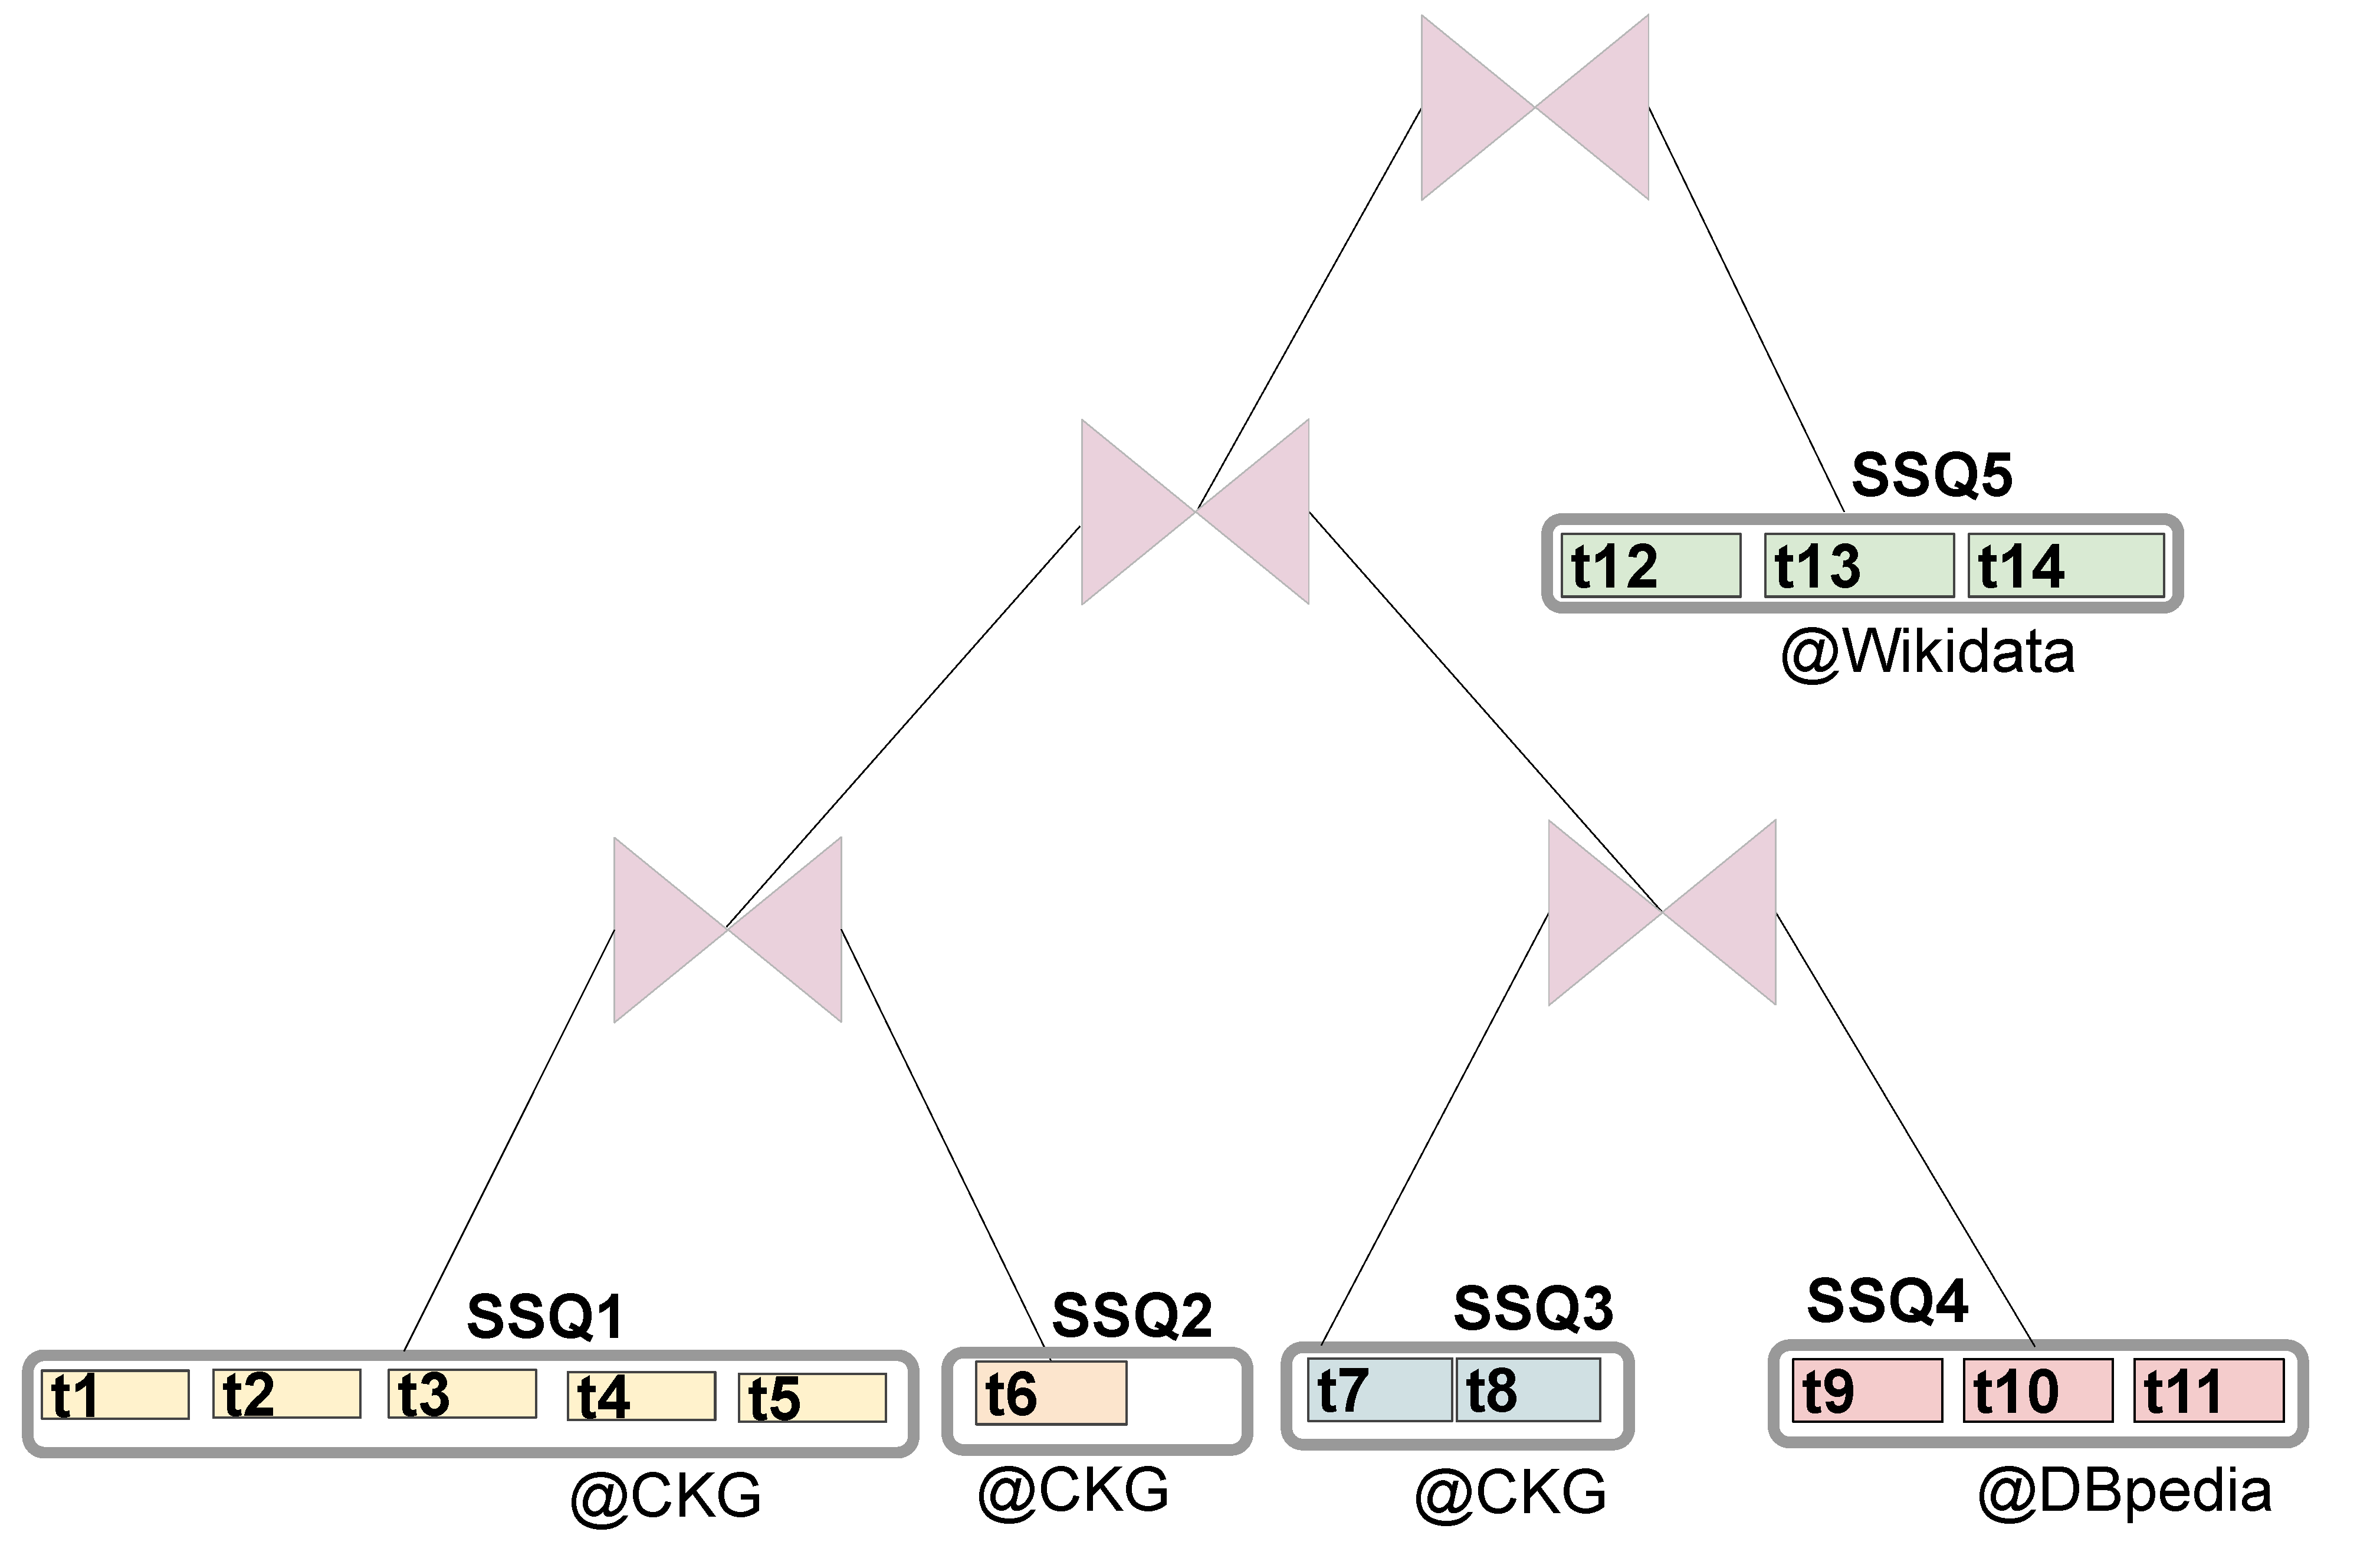
\includegraphics[width=0.50\textwidth]{figs/QueryPlanB.pdf}}
\caption{\textbf{Federated query.} a) SPARQL query comprising 14 triple patters to be executed over a federation including Cancer Knowledge Graph (CKG), DBpedia, and Wikidata. b) A query plan composed of five star-shaped subqueries SSQ1, SSQ2, SSQ3, SSQ4, and SSQ5 corresponding to the query decomposition. 
Each SSQ is executed over the graph that can answer the SSQ. The execution engine follows the query plan; the execution of four joins merges the SSQ answers and produces the federated query answer.}
\label{fig:federatedQuery}
\end{figure}

\arxivonly{The problem of query execution is defined in terms of data shipping strategies that are able to distribute query load between a server-client architecture of Linked Data Fragments.
State of the art approaches tackle this issue by employing graph partitioning techniques to generate graph pattern fragments.
These fragments aim to improve query performance, scalability, and workload balance. 
SAGE~\cite{DBLP:conf/f-ic/MinierSM19}, smart-KG~\cite{DBLP:conf/www/AzzamFABP20}, brTPF~\cite{DBLP:journals/corr/HartigA16}, SkyTPF~\cite{DBLP:conf/semweb/KelesH19}, SPF~\cite{DBLP:journals/corr/abs-2002-09172}, TPF~\cite{DBLP:journals/ws/VerborghSHHVMHC16}, and WiseKG~\cite{DBLP:conf/www/AzzamAMKPH21} are exemplary approaches for accessing graph patterns of varying shapes.
These interfaces for Linked Data Fragments may significantly accelerate query execution, reduce workload, and minimize data transfer.
Moreover, query rewriting based on these fragments correctly produces all the answers of the rewritten query, i.\,e., the methods are sound and complete.
However, it is important to note that there exists a trade-off between memory consumption and execution time improvement so that storage requirements (e.\,g., smart-KG) can be twice as high in comparison to other approaches (e.\,g., SAGE, TPF, or SPF), due to the need to store partitions and their associated metadata. 

Because of the variety of available interfaces, some works have proposed methods for heterogeneous federations~\cite{DBLP:conf/www/HelingA22,DBLP:conf/semweb/MontoyaKH19,DBLP:conf/semweb/MontoyaAH18a,DBLP:conf/esws/ChengH22}, where the goal is to find efficient query execution plans in consideration of the constraints as well as strengths of the available interface.}

\section{Trustworthiness and Provenance of Graph Data}
\label{sec:trustprovenance}
Trustworthiness of web pages and data on the web can be detected by various indicators, e.\,g., by certificates, by the placement of search engine results, and by links (forward and backward links) to other pages.
However, on the Semantic Web, there are few ways for users to assess the trustworthiness of individual data. 
Rules can be utilized to define policies and business logic over the web of data, and transparently used to infer data that validate or do not validate these policies.
The trustworthiness of inferred data can be assessed through its provenance, which encompasses metadata detailing how the data was acquired and verified~\cite{DBLP:conf/rr/KhandelwalJK11}.

The trustworthiness of data on the web can be inferred from the trustworthiness of other users (``Who said that?''), the temporal validity of facts (``When was a fact described?''), or in terms of uncertainty of statements (``To what degree is the statement true?'').
Artz and Gil~\cite{DBLP:journals/ws/ArtzG07} summarize trustworthiness as follows:
``Trust is not a new research topic in computer science, spanning areas as diverse as security and access control in computer networks, reliability in distributed systems, game theory and agent systems, and policies for decision-making under uncertainty. The concept of trust in these different communities varies in how it is represented, computed, and used.''
Although trustworthiness has long been considered in these areas, the provision and publication of data by many users to multiple sources on the Semantic Web introduces new and unique challenges.

One way of facilitating trust on the Semantic Web is to capture and provide the provenance of data with the PROV ontology (PROV-O)\footnote{\url{https://www.w3.org/TR/prov-o/}}.
It captures information about which \emph{Agents} cause data \emph{Entities} to be processed by which \emph{Activities}.
Capturing such information requires the use of known tools for modeling metadata for RDF data, e.\,g., reification, singleton properties, named graphs, or RDF-star\footnote{\url{https://w3c.github.io/rdf-star/}}.
While some approaches use these constructs to capture provenance information for each triple individually~\cite{DBLP:conf/semweb/GalarragaMH17}, 
others exploit the fact that typically multiple triples share the same provenance~\cite{DBLP:conf/semweb/HansenLGLTH20} so that they can be combined into the same named graph encoding the provenance information only once for a set of triples.
Delva et al.~\cite{DBLP:conf/edbt/DelvaDJB23} introduce the notion of shape fragments, which entail the validation of a given shape through the neighborhood of a node, along with the node's provenance and the rationale behind its validation.

Furthermore, trustworthiness also plays a role in inference services on the Semantic Web, as data inference must consider specifications related to trustworthiness and data must be evaluated for trustworthiness.
Important aspects for trustworthiness of data include~\cite{DBLP:journals/ws/ArtzG07}:
the origin of the data, 
trust already gained based on previous interactions, 
ratings assigned by policies of a system, and 
access controls and, in some cases, security and importance of information.
These aspects are realized in different systems.

In general, data provenance and trustworthiness of data on the Semantic Web have been addressed for RDF data \cite{DBLP:journals/ki/DividinoSSS09,DBLP:conf/semweb/FlourisFPTC09} as well as for OWL and rules in \cite{DBLP:journals/ki/DividinoSSS09}.
In addition, there are some recent approaches on supporting how-provenance for SPARQL queries~\cite{DBLP:journals/jacm/GeertsUKFC16,DBLP:journals/pvldb/HernandezGH21,DBLP:conf/www/Galarraga0KH23} with the goal of providing users with explanations on how the answers to their queries were derived from the underlying graphs.
Other work deals with access controls over distributed data on the Semantic Web~\cite{DBLP:conf/esws/GavriloaieNOSW04}.
Furthermore, there are approaches to computing trust values~\cite{DBLP:journals/jair/StoilosSPTH07} and informativeness of subgraphs~\cite{DBLP:conf/cikm/KasneciEW09}.
There are also digital signatures for graphs~\cite{DBLP:conf/ecai/BellomariniNS20}.
Analogous to digital signatures for documents, entire graphs or selected vertices and edges of a graph are provided with a digital signature to ensure the authenticity of the data and thus detect unauthorized modifications~\cite{DBLP:phd/dnb/Kasten16}.
In the approach for digital graph signatures developed by Kasten et\,al., graph data on the Web is supported in RDF format as well as in OWL~\cite{DBLP:conf/esws/KastenSS14}.
The digital graph signature is itself represented as a graph again and can thus be published together with the data on the Web.
The link between the signature graph and the signed graph is established by the named graph mechanism~\cite{DBLP:conf/esws/KastenSS14}, although other mechanisms are also possible.
Through this mechanism, it is possible to combine and nest signed graphs.
It is thus possible to re-sign already signed graphs together with other, new graph data, etc.
This makes it possible to build complex chains of trust between publishers of graph data and to be able to prove the origin of data~\cite{DBLP:conf/esws/KastenSS14,DBLP:phd/dnb/Kasten16}.

\section{Applications}
\label{sec:userinterfaces}
\label{sec:examples}

With the increasing spread and use of semantic and linked data on the Web, the requirements for Semantic Web applications have increased at the same time as their application possibilities.
The general requirements for applications based on semantic data on the Web are given by their flexible and diverse representation and descriptions.
Applications that use data from relational databases or XML documents can start from a fixed schema. 
However, this cannot be assumed for data on the Web. 
Often, neither the data sources nor the type and amount of data in a source are fully known.
The dynamics of semantic data on the Web must be taken into account by applications accordingly, both when querying and aggregating data, and when visualizing data.
Thus, the real challenge of Semantic Web applications is to guarantee the best possible flexibility of the application to take into account the dynamics of data sources, data, and schemas during input, processing, and output.

In the following, selected examples of Semantic Web applications or application areas are presented. 
They illustrate how flexibility and quality of search, integration, aggregation, and presentation of data from the Web can be implemented. 
At the same time, they show the potential of Semantic Web applications.
First, uniform vocabularies and schemas are presented using the example of \textit{schema.org}.
These serve as a basis for semantic search to provide search engines with information about the meaning of web document content.
The search and integration of data from different sources is supported by \textit{Sig.ma}, a semantic web browser.
Other applications provide semantic search through other representation formalisms, e.\,g., \textit{Knowledge Graphs}).
Subsequently, the \textit{Facebook Graph-API}, an application programming interface (\textit{API}) to the Facebook (Knowledge) Graph, is introduced.

\subsection{Vocabularies and Schemas: Schema.org}

In HTML documents, the structure and composition of pages can be described with tags, but not the meaning of the information.
Vocabulary, schemas, and microdata can be used as mark-up in HTML documents to describe information about page content and its meaning in a way that search engines can process this information.

Schema.org\myurl{http://schema.org} is a collection of vocabularies and schemas to enrich HTML pages with additional information.
The vocabulary of \textit{Schema.org} includes a set of classes and their properties. A universal class ``thing'' is the most general, which is a kind of umbrella term for all classes.  
Other common classes are \textit{Organization}, \textit{Person}, \textit{Event}, and \textit{Place}.
Properties are used to describe classes in more detail.
For example, a person has the properties such as name, address, and date of birth.

In addition to vocabularies, Schema.org also specifies the use of HTML microdata, with the goal of representing data in HTML documents in as unambiguous a form as possible so that search engines can interpret it correctly.
An example of this is formats for unique dates and times, which can also describe intervals to indicate the duration of events.

Schema.org is supported by the search engines Bing, Google, and Yandex, among others.
There are extensions and libraries for various programming languages, including PHP, JavaScript, Ruby, and Python, to create web pages and web applications using vocabularies and microdata from Schema.org. 
Likewise, there are mappings from Schema.org vocabularies and microdata to RDFS.

\subsection{Semantic Search}

A classic web browser enables the display of web pages.
A semantic web browser goes one step further by additionally allowing the user to visualize the underlying information of individual pages, for example in the form of RDF metadata. 
Semantic Web browsers are also referred to as hyperdata browsers because they allow navigation between data while also allowing one to explore the connection to information about that data.
Thus, ordinary users can use and exploit Semantic Web data for their information search.

Sig.ma~\cite{key:sigma} was an application for (browsing) Semantic Web data, which may come from multiple distributed data sources.
Sig.ma provided an API for automatically integrating multiple data sources on the Web.
The requested data sources describe information in RDF.
A search in Sig.ma was initiated by a textual query from the user.
Entities such as people, places, or products can be searched for.
Results of a query are presented in aggregated form, that is, properties of the searched entity, such as a person, are presented in aggregated form from different data sources. 
For example, in a person search, information such as e-mail address, address, or current employer can be displayed.
In addition to the actual information, links to the underlying data sources are also displayed to allow users to navigate to refine their search.
Sig.ma also supported structured queries in which specific characteristics can be requested for an entity, such as contact information for a specific person.

Queries to data sources occur in parallel. 
The results from each data source in the form of RDF graphs are summarized by using properties of links in RDF data, such as \texttt{owl:sameAs}, or inverse-functional predicates.
When searching data sources, techniques such as indexes, logical inference, and heuristics are used for data aggregation.
OntoBroker\myurl{https://www.semafora-systems.com/ontobroker-and-ontostudio-x}~\cite{Decker1999} and OntoEdit~\cite{10.1007/3-540-48005-6_18} are ontology editors with search and inference systems for ontologies. 
Using OntoBroker, complex queries over distributed Semantic Web resources, e.\,g., represented in OWL, RDF, RDFS, SPARQL, and also F-Logic) can be efficiently processed.

\subsection{Knowledge Graphs and Wikidata}

There is an increasing number of knowledge bases and representations of structured data.
For example, the secondary database Wikidata\myurl{https://www.wikidata.org/wiki/Wikidata:Introduction/de}~\cite{DBLP:journals/cacm/VrandecicK14}.
A secondary database includes, in addition to the (actual) statements, relationships to their sources and other databases (called secondary information). 
Wikidata is a shared database between Wikipedia and Wikimedia. 
Wikidata mainly contains a collection of objects, which are represented as triples over the objects' properties and the corresponding values. 
Semantic MediaWiki\myurl{https://www.semantic-mediawiki.org/wiki/Semantic_MediaWiki} is an extension of MediaWiki. 
It serves as a flexible knowledge base and knowledge management system. 
Semantic MediaWiki extends a classic wiki with the ability to enrich content in a machine-readable way using semantic annotations. 
  
Another knowledge base was Freebase\myurl{https://www.freebase.com}, also an open and collaborative platform initiated in 2007 and acquired by Google in 2010.
The content from Freebase was taken from various sources, including parts from the MusicBrainz ontology mentioned earlier.
The success and widespread use of Wikidata prompted Google to migrate Freebase to Wikidata~\cite{DBLP:conf/www/TanonVSSP16}.
This strengthened the goal to develop a comprehensive, collaborative basis of structured data.

Google offers a semantic search function with Google Knowledge Graph\myurl{http://www.google.com/insidesearch/features/search/knowledge.html}$^,$\myurl{https://developers.google.com/knowledge-graph/}.
A knowledge graph, like an RDF graphs, is a set of triples representing links between entities.
This forms a semantic database.
Possible entity types are described on schema.org, among others.
If a search term occurs in a query, the corresponding entity is searched for in the knowledge graph. 
Starting from this entity, it is then possible to navigate to further entities by means of the links. 

\subsection{API-Access to Social Networks} 

A social network is essentially a graph in which connections are formed from users to other users, e.\,g., in the form of a friendship relationship or to events and groups.
Facebook's Graph API describes a programming interface to the Facebook Graph (called \textit{Open Graph}).
Within the graph, people, events, pages, and photos are represented as objects, with each object having a unique identifier.
For example, \url{https://graph.facebook.com/abba} is the identifier of ABBA's Facebook page.
There are also unique identifiers for the possible relationship types of an object, which allow navigating from one object to all connected objects with respect to a particular relationship.

The Graph API allows one to navigate the Facebook Graph and read objects, including their properties and relationships to other objects, as well as creating new objects in the Facebook Graph and deploying applications.
The API also supports requests for an object's metadata,
such as \textit{when} and \textit{by whom} an object was created.

\section{Impact for Practitioners}
\label{sec:praxis}
\label{sec:impact}

Linking and using graph data on the Web has become a widespread practice. 
Today, there is a large amount of open data in various formats and domains, such as bibliographic information management, bioinformatics, and e-government.
DBpedia is the central hub in this context, around which different datasets and domains are grouped (cf.~\cite{DBLP:journals/expert/Bizer09}).
This is illustrated, e.\,g., by the tremendous growth of the Linked Open Data Cloud\footnote{The growth of the Linked Open Data Cloud is documented at: \url{http://linkeddata.org/}.} since 2007.
Two of the latest notable supporters of graph-based data are online auctioneer eBay with their graph database\footnote{\url{https://github.com/eBay/akutan}} and the U.S. space agency NASA with the unification of internal distributed case databases as knowledge graphs\footnote{\url{https://blog.nuclino.com/why-nasa-converted-its-lessons-learned-database-into-a-knowledge-graph}}.
These and other success stories of the Semantic Web in industries and industry-scale knowledge graphs are described by Noy et al.~\cite{DBLP:journals/cacm/NoyGJNPT19}.
Further analyses and surveys arguing about the importance but also challenges of using graph data can be found in the literature like the 2020 survey of Sahu et al.~\cite{DBLP:journals/vldb/SahuMSLO20} and the 2021 reflection about the future of graphs by Sakr et\,al.~\cite{DBLP:journals/cacm/SakrBVIAAAABBDV21}.
The usefulness of knowledge graphs and semantic-based data modeling for complex systems is also discussed in the 2024 book by Abonyi et al.~\cite{AbonyiEtAl2024OntologiesInIndustry}.
\arxivonly{The importance of graph databases is also reflected by the Forbes business magazine, which predicted in 2019 that graph databases would be the next mainstream database technology\footnote{\url{https://www.forbes.com/sites/cognitiveworld/2019/07/18/graph-databases-go-mainstream}}.}

Regarding lightweight open graph data, Schema.org defines schemas for modeling data on web pages to provide information about the underlying data structures and meaning of the data.
Search engines can use this additional information to better analyze the content of web pages.
As mentioned above, Schema.org is supported by search engines such as Bing, Google, and Yandex. 
Studies on selected sources have shown that web pages among the top 10 results have up to 15~\% higher click-through rate\footnote{\url{http://developer.yahoo.net/blog/archives/2008/07/}}.
Other companies like BestBuy.com even report up to 30~\% higher click-through rates since adding semantic data to their websites (cf.~Section~\ref{sec:userinterfaces}) in 2009.
BestBuy.com uses the GoodRelations vocabulary\myurl{http://www.heppnetz.de/projects/goodrelations/} to describe online offers.
Similarly, Google uses semantic data from online commerce portals that use the GoodRelations vocabulary and takes it into account when searching\footnote{\url{http://www.ebusiness-unibw.org/wiki/GoodRelationsInGoogle}}. 

Another success is the publication of government data.
For example, the U.S. government makes government data publicly available with data.gov\myurl{http://www.data.gov/}, and U.S. Census\myurl{http://www.rdfabout.com/demo/census/} publishes statistical data about the United States.
In the UK, data.gov.uk\myurl{http://data.gov.uk} is a key part of a program to increase data transparency in the public sector.
The European Commission operates data.europa.eu\myurl{https://data.europa.eu/}, a European data portal with metadata about the member states.
Among others, it provides a SPARQL endpoint to access the data.

Finally, a strong growth of semantic biomedical data on the Web can be noted.
As part of Bio2RDF\myurl{http://bio2rdf.org/}, many bioinformatics databases have been linked.
Transinsight GmbH offers the knowledge-based search engine GoPubMed\myurl{http://www.gopubmed.org/} to find biomedical research articles.
Ontologies are used for searching.

Regarding more heavyweight ontologies in OWL, there has also been movement in recent years. 
In addition to numerous research-derived inference engines such as Pellet and Hermit mentioned above, inference mechanisms for OWL can now be found in commercial graph databases such as neo4j\footnote{\url{https://neo4j.com/blog/neo4j-rdf-graph-database-reasoning-engine/}}.
Furthermore, pattern-based core ontologies can also be found in software development workflows~\cite{DBLP:conf/semweb/SchonteichKS18}.
The development and use of core ontologies is part of a continuous delivery process that is used in practice.

\section{Summary and Outlook}

The Semantic Web consists of a variety of techniques that have been heavily influenced by long-term artificial intelligence research and its results.
The current state is also driven by an industry uptake under the umbrella term of Knowledge Graphs and reflected in various activities as described.
In summary, therefore, it can be observed that semantic data on the Web is having a real impact on commercial providers of products and services, as well as on governments and public administrations.

Despite all the research and industrial developments, the full potential of the Semantic Web has not yet been exploited.
Some important components of the Semantic Web architecture are still being explored, such as data provenance and trustworthiness.
Below, we describe three example directions for future work.
\begin{itemize}
    \item Neuro-symbolic systems: As mentioned in the introduction, we see as an important direction of future work the combination of symbolic AI and subsymbolic AI.
    By combining the strength of Large Language Models (LLM), i.\,e., generative AI, in processing and generating natural language text and accessing structured data and logical reasoning capabilities of the Semantic Web, a next step towards the vision of automated agents that perform complex planning tasks may be reached.
    An example is performing A* search with an LLM~\cite{DBLP:journals/corr/abs-2310-13227-toolchainstar}.
 Specifically, LLMs might comprehensively capture and acquire human knowledge~\cite{10.1145/3608966}, but current LLMs lack responding to simple questions of non-existing facts in their training data~\cite{10.1145/3608966}, may not contain all facts~\cite{DBLP:journals/corr/abs-2308-10168}, and thus return less accurate answers~\cite{Hou2023-fo}.
To leverage the distinct capabilities of both LLMs and the Semantic Web, the integration of neuro-symbolic systems appears to offer a viable solution~\cite{DBLP:journals/corr/abs-2306-08302}. 
Neuro-symbolic systems could also address the problem that LLMs' output is based on the most probable answer, which sometimes leads to wrong answers -- often referred to as ``hallucinations''~\cite{DBLP:journals/corr/abs-2302-04023,DBLP:conf/adbis/Hose23,DBLP:journals/corr/abs-2308-10168}. 
    \item Natural interfaces between machine and users: 
    A key to successful applications of the Semantic Web is intuitive user interfaces.
    Users must be offered applications that are intuitive and easy to use.
    This includes improving interfaces based on natural language for formulating queries and accessing structured data stored in SPARQL endpoints.
    Again, the use and deeper integration of LLMs with Knowledge Graphs shows a promising direction.
    \item Semantic Web components: There are still components of the architecture (see Section~\ref{sec:swarchitecture}) where active development and research are conducted.
    Most notably, there are crypto and trust. 
    Recent new W3C standards such as DID and Verifiable Credentials have been developed. 
    However, one can expect more work and development in this direction.
\end{itemize}

Finally, we like to point to existing literature discussing the future directions of research on the Semantic Web~\cite{DBLP:journals/corr/abs-2309-13939} and Knowledge Graphs~\cite{DBLP:journals/corr/abs-2308-14217}.
Breit et al. \cite{10.1145/3586163} conducted a survey on the fusion of Semantic Web and Machine Learning, exploring the opportunities arising from the convergence of these two paradigms.

\subparagraph*{Acknowledgements}

This article is a living document.
The first version was written by Jannik, Scherp, and Staab in 2011~\cite{DBLP:journals/insk/JanikSS11}.
It was translated to German and updated by Gröner, Scherp, and Staab in 2013~\cite{DBLP:books/ol/13/GronerSS13} and updated again by Gröner and Scherp in 2020~\cite{DBLP:books/degruyter/20/ScherpG20}.
This release in 2024 reflects on the latest developments in knowledge graphs and large language models.

\bibliography{tgdkbib}

\end{document}
